%% inicio, la clase del documento es iccmemoria.cls
\documentclass{iccmemoria}

\setcounter{secnumdepth}{4}
\setcounter{tocdepth}{4}

%% datos generales y para la tapa
\titulo{Evasión de obstáculos con flujo óptico y redes neuronales para vehículos aéreos no tripulados}
\author{Jorge Gómez Valderrama}
\supervisor{Matthew Bardeen}
\informantes
	{Profesor Informante 1}
	{Profesor Informante 2}
\adicional{(sólo por si se necesita agregar algún otro profesor)}
\director{Profesor del ramo Memoria de Título}
\date{mes, año}

%% inicio de documento
\usepackage{graphicx}
\begin{document}

%% crea la tapa
\maketitle

%% dedicatoria
\begin{dedicatory}
Dedicado a ...
\end{dedicatory}

%% agradecimientos
\begin{acknowledgment}
Agradecimientos a ...
\end{acknowledgment}

%% indices
\tableofcontents
\listoffigures
\listoftables
\listofalgorithms

%% resumen
\begin{resumen}
Aquí va el resumen (en Castellano)... 
\end{resumen}

%% abstract

%% contenido del primer capítulo
\chapter{Introducción}

\section{Descripción del contexto}

La motivación para trabajar en este tema viene de ven que en la naturaleza existe gran variedad de animales que pueden alzar vuelo y de cómo estos tienen total control sobre las maniobras que pueden hacer. Entonces si se comprende cómo logran hacer esto se podría aplicar esos mismos mecanismos a los vehículos aéreos no tripulados.\\

Una de las formas en que la aves dirigen su vuelo es por medio del flujo óptico, con esto logran extraer información de la escena en que encuentran y así navegar a través de esta. La información es obtenida por medio de la visión la que luego es procesada en el cerebro \cite{bhagavatula2011optic}.\\

Con la intención de hacer un símil con la naturaleza, se toma como modelo el uno de los mecanismos que tienen las aves para dirigir el vuelo y se traspasa a los vehículos aéreos no tripulados. Todo esto por medio del flujo óptico y redes neuronales.\\

Cuando se habla de un vehículo aéreo no tripulado (también conocidos como drones) se hace mención a cualquier tipo de aeronave que no tenga un piloto a bordo. Sin embargo en el contexto de este documento se hace referencia a un tipo específico de aeronave los cuadricópteros, los que son un tipo de multirrotor, véase sección \ref{sec:uav}.\\

En los últimos años este tipo de aeronaves han ganado mucha popularidad, debido al avance de la tecnología, producción a una mayor escala y precios más reducidos. Si bien en un principio eran empleados en áreas militares y técnicas ahora son usados en una gran variedad de campos distintos. La una de las razones principales por lo que ahora  los cuadricópteros son usados ampliamente es por uno de sus componentes principales, el controlador de vuelo. El cual tiene como función principal controlar los motores de tal manera que permite mantener a los multirrotores en aire de forma estable.\\

Estas caracteristicas permiten que controlar estas aeronaves sea una tarea más sencilla, automatizando varios aspectos del vuelo, permitiendo que ahora cualquier persona pueda volar un cuadricóptero. Pero a pesar de esto hay ámbitos en los cuales todavía tiene que hacerse cargo el piloto, como lo es la reacción ante objetos que se interpongan en la trayectoria de vuelo. Este es un campo en cual todavía se necesita investigación y desarrollo.\\

%Por otro lado si buscamos antecedentes donde esta problemática está resuelto nos encontramos con múltiples ejemplos en la naturaleza. Es posible encontrar una gran variedad de animales que tiene la cualidad de alzar vuelo y sortear las mismas complicaciones a las que se enfrentan los cuadricópteros. Uno de los mecanismos que los pájaros utilizan es la percepción de flujo óptico a través de la visión y posterior procesamiento en el cerebro para detectar y evadir obstáculos, lo que conlleva a poder dirigir su vuelo \cite{bhagavatula2011optic}.\\

%Por los antecedentes mencionados anteriormente se intenta tomar el concepto de ciertos modelos biológicos y usarlos como base para crear un sistema que tiene la finalidad de imitar el comportamiento animal para resolver el problema expuesto.\\

\section{Definición del problema}

Los cuadricópteros tiene la capacidad de mantenerse en vuelo sin la intervención de un piloto, ya sea sobre una posición específica o siguiendo una ruta programada, esto es posible gracias al controlador de vuelo que cada multirrotor tiene a bordo. Este controla cada movimiento que realiza y puede llegar a hacer muchas tareas de forma autónoma, como lo es despegar, aterrizar o desplazarse a un punto en específico en el aire.\\
 
Las prestaciones mencionadas son realizadas por la adición de dispositivos al controlador de vuelo, estos le entregan información en distintos ámbitos, la que puede ser la posición georeferenciada mediante GPS, la altura por la medición barométrica, los movimientos que realiza el cuadricóptero con sensores de aceleración lineal y angular (acelerómetros y giroscopios), entre otros.\\
 
Si bien con toda la información que el controlador de vuelo puede recopilar del entorno, las funciones que este puede cumplir de forma autónoma tiene un paradigma proactivo, es decir, estas deben ser planeadas en detalle de antemano, por ejemplo: si se requiere que el cuadricóptero siga una determinada ruta conformada por puntos de GPS, es necesario diseñar esta de tal forma que no interfiera con algún elemento con el que este puede colisionar.\\
 
Es por este motivo que las aplicaciones de conducción autónoma se realizan en espacios abiertos donde exista poca intervención del entorno, pero si se requiere que estos vuelen en espacios más confinados o donde falla la asistencia de georreferencia por ejemplo, se debe hacer un vuelo manual asistido por un piloto.\\
 
Entonces la carencia que presentan los multirrotores es la capacidad de ser reactivos ante eventos que ocurran en el entorno, si pudieran reaccionar frente a estos, sin ser previstos de antemano al momento de planificar el vuelo, los cuadricópteros podrían ampliar su rango de aplicaciones.\\
 
La falencia está en que no existe un sistema que proporcione una comprensión del entorno donde se realiza el vuelo y que permita tomar decisiones frente a eventualidades que puedan ocurrir durante este.\\

\section{Propuesta de solución}

Para solventar la falencia mencionada anteriormente se propone implementar un sistema que permita la detección de obstáculos y la evasión de estos, de esta forma agregar al cuadricóptero una herramienta que le permita enfrentar este tipo de problemáticas.\\

La información de objetos será capturada por medio de una cámara digital, el video entregado por esta se procesara para obtener el flujo óptico presente en las imágenes, véase sección \ref{flujo_optico}, éste permite rescatar datos de donde se encuentran los objetos dentro de la imagen.\\

Una vez que se obtenga el flujo óptico, será entregado a una red neuronal, véase seccion \ref{redes_neuronales}, la que dara como salida la dirección a la cual se debe hacer un movimiento para evadir un obstáculo.\\

\section{Objetivos}

En esta seccion de describe los elementos que son necesarios desarrollar para poder dar solucion al problema. Se menciona el objetivo general y que se necesita para este se pueda satisfacer, ademas de dar a conocer las limitaciones del sistema a implementar.

\subsection{Objetivo general}

Implementar un sistema que sea capaz de detectar obstáculos y entregar la información necesaria de como evadirlos, mediante flujo óptico y redes neuronales.

\subsection{Objetivos específicos}
 
\begin{itemize}
    \item Definir herramientas que permitan la obtención de flujo óptico desde la captura de video.
    \item Implementación de una red neuronal que permita el procesamiento del flujo óptico.
    \item Entrenamiento de una red neuronal para que sea capaz de aprender cómo evadir obstáculos.
    \item Implementación de un robot omnidireccional que permite la obtención de datos para entrenar la red neuronal.
    \item Realizar pruebas con el robot para evaluar el comportamiento de la red neuronal ante obstáculos.
\end{itemize}
 
\section{Alcances}
 
\begin{itemize}
    \item El sistema será probado con un robot omnidireccional que solo puede moverse en un plano de dos eje.
    \item La evasión de obstáculos solo se realizará en un eje.
    \item Solo se evadirán objetos estáticos y de uno a la vez.
    \item Las pruebas serán realizada en una pista diseñada con este fin bajo condiciones controladas.
\end{itemize}

En este capítulo se describió las razón por las que se aborda esta temática, mencionando el interés que se tiene de imitar los mecanismos que se encuentran en la naturaleza para dirigir el vuelo y utilizarlos en los vehículos aéreos no tripulados. También se definió la problemática y como se pretende solucionar, en particular la detección y posterior evasión de obstáculos por medio del flujo óptico y redes neuronales. Además de describir los objetivos que se necesitan cumplir para dar con la solución.\\

%% contenido del segundo capítulo
\chapter{Marco teórico}

En este apartado se describen elementos que son necesarios para la comprensión del problema y la implementación de la solución. Se detalla que es un cuadricóptero, como este se mueve en el aire y por qué es importante para la implementación. Se profundiza en la teoría del software a utilizar, lo que abarca: visión por computador; flujo óptico, su definición y cómo es posible calcularlo; redes neuronales, que son, como funcionan y aprenden. Del hardware se introduce a los robot omnidireccionales y algunos elementos que se utilizan en la construcción de este, que son microcontrolador, controlador de motores y el sensor óptico de movimiento.\\

\section{Vehículo aéreo no tripulado}\label{sec:uav}

La problemática descrita fue obtenida de los vehículos aéreos no tripulados, por lo que importante describir que son y qué elementos de estos son importantes para a tomar en cuenta en la solución propuesta.\\

Un vehículo aéreo no tripulado, UAV (por sus siglas del inglés: \emph{unmanned aerial vehicle}) o dron, es cualquier aeronave que no cuente con un piloto o tripulación a bordo, por lo que ésta puede volar de forma autónoma por medio de un computador a bordo o ser controlada remotamente por un humano \cite{icao2011UAS}.\\

Dentro de los vehículos aéreos no tripulados se encuentran los multirrotores o multicópteros, estas son aeronaves que generan sustentación por medio del giro de alas o hélices sobre un eje, siendo este conjunto llamado rotor. La Organización de Aviación Civil Internacional (CIAO por sus siglas del inglés: \emph{International Civil Aviation Organization}) los define como aeronaves que se mantienen en vuelo por las reacción del aire en uno o más rotores. En el caso de los multirrotores estos están compuestos por dos o más rotores, se diferencian de los helicópteros en la forma que logran el control y la estabilidad, estos tienen mecanismos que varían el paso de las hélices modificando su ángulo de ataque, en cambio los multirotores lo hacen por medio del cambio de velocidad relativa de cada rotor, produciendo cambios en el empuje y torque.\\

Un tipo de mutirrotor son los cuadricópteros los cuales tiene dos pares de rotores con hélices iguales y paso fijo, dos giran en sentido horario y los otros dos en sentido antihorario, esta configuración permite que el torque de cada rotor se anule con el rotor correspondiente que gira en sentido contrario, de esta forma el cuadricóptero se estabiliza y no gira sobre su propio eje \cite{AllenQuadcopters}.\\

Se describe este tipo de UAV porque la solución a entregar va a enfocada a este grupo de aeronaves, principalmente a los cuadricópteros que bordean los 250 mm de diámetro.\\  

Como se mencionó anteriormente los movimientos de los multirrotores se logran variando la velocidad de cada rotor independientemente, referencia a la imagen, con esto el cuadricóptero puede moverse sobre 3 ejes perpendiculares, por medio de los movimientos de \emph{pitch}, \emph{roll} y \emph{yaw}, además de desplazarse por el eje $Z$ variando su altitud.\\

Con el movimiento \emph{pitch} el cuadricóptero rota sobre el eje $X$ y se desplaza hacia adelante o atrás por el eje $Y$, cuando ejecuta el movimiento de \emph{roll} rota sobre el eje Y y se desplaza de izquierda a derecha sobre el eje $X$ y gira sobre el eje $Z$ con el movimiento de \emph{yaw}. Con esto se logra tener control sobre 4 grados de libertad.\\

Es necesario saber cómo son capaces de moverse los cuadricópteros, ya que en las pruebas a realizar se busca imitar los movimientos que estos realizan. De esta forma al capturar video se tenga una visión muy cercana a la que se tendría al hacerlo desde un cuadricóptero. Con la limitación de que el movimiento solo es realizado en dos ejes sobre una superficie, por medio de un robot omnidireccional, véase sección \ref{omni_robot}.\\

\section{Visión por Computador}

\emph{Computer Vision} (visión por computador) es una disciplina que busca que los computadores puedan tener una comprensión de alto nivel sobre imágenes o videos digitales, por ejemplo, con el objetivo de automatizar tareas que el sistema visual humano ya puede hacer\cite{ballard1982computer, vandoni1996proceedings, sonka2008image}.\\

Dentro de las tareas de la visión por computador están: la adquisición, procesamiento, análisis, el entendimiento de imágenes digitales y la extracción de información multi dimensional del mundo real, para producir información numérica o simbólica \cite{klette2014concise, shapiro2001computer, morris2004computer, forsyth2003computer}.\\

Dado que nosotros percibimos el mundo principalmente por medio de la vista, parecería sencillo traspasar nuestra experiencia a la visión por computador, pero en realidad es una tarea muy difícil, debido a la complejidad de cómo funciona nuestro cerebro. Contamos con múltiples sistemas que reciben distinta información segmentada desde el sistema visual e incluso otros sistemas, pero en el caso de la visión por computación solo contamos con una imagen (en el caso de video una secuencia de imágenes) y esto es todo lo el computador puede \emph{"ver"}.\\

Cuando hablamos de una imagen nos estamos refiriendo a la información que nos es capaz de entregar la luz que es recibida desde el entorno o una escena. Esta información varia dependiendo del contexto en que se hable, si nos referimos a un marco biológico la luz incidirá en un ojo y las células en la retina generaran las señales eléctricas que el cerebro interpretará como imágenes, si hablamos de una cámara la imagen se formará en una película fotografica o en un sensor digital \cite{bradski2008learning}.\\

Dado el ámbito de este documento, es preciso profundizar en las imágenes digitales, esta puede ser definida como la integración y muestreo de información analógica (luz incidiendo en un sensor fotográfico) en un dominio espacial. Esta consiste en un arreglo rectangular de pixeles $(x, y, u)$, cada uno contiene una ubicación $(x, y) \in \mathbb{Z}^2 $ y un valor $u$, muestreado en una ubicación $(x, y)$. $\mathbb{Z}$ es conjunto de puntos $(x, y)$ del arreglo rectangular \cite{klette2014concise}. Entonces podemos definir una imagen como:
\begin{equation}
	\begin{split}
	I = \lbrace (x, y) : 1 \leq  x \leq N_{cols} \wedge 1 \leq y \leq N_{rows} \rbrace \subset \mathbb{Z}^2
	\end{split}
\end{equation}

\section{Flujo óptico}\label{flujo_optico}

El flujo óptico es uno de los elementos centrales en este documento. Es obtenido por medio del procesamiento de imágenes, con el fin de obtener información de la escena circundante. Esta informacion es la que será utilizada por la red neuronal posteriormente. En esta sección se describe que es el flujo óptico y como es calculado.\\

El flujo óptico es definido como el cambio de la estructura de la luz en una imagen, por ejemplo, en la retina de un ojo o en el sensor de una cámara, debido a movimiento relativo del observador y escena. Cuando los objetos se mueven frente a una cámara o esta se mueve en un entorno fijo, existe un cambio correspondiente a los movimientos en la imagen, estos cambios pueden utilizarse para recuperar información relativa al movimiento de las formas y los objetos.\\

Podemos definir un campo de movimiento, en el cual asignamos un vector de velocidad a cada punto de la imagen. En un instante en particular, un punto $P_i$ en la imagen corresponde con algún punto $P_0$ en la superficie de un objeto. Los dos puntos son conectados por la ecuación de proyección. Si consideramos una proyección de perspectiva, una línea se extiende de un punto en la imagen, pasa por el centro de la lente (en el caso de tratarse de una cámara), hasta un punto en la superficie de la escena.\\


\begin{figure}[H]
  \centering
  \includesvg[width = 300pt, svgpath = images/proyeccion_flujo_optico]{}
  \caption[Proyección de un punto sobre la imagen.]{Proyección de un punto $P_0$ con movimiento $v_0$ en la escena  a un punto $P_i$ con movimiento $v_i$ sobre la imagen.}
  \label{fig:proyeccion_flujo_optico}
\end{figure}

El punto $P_{0}$ tiene una velocidad $v_{0}$ relativa a la cámara, esto induce un movimiento $v_{i}$ en el punto $P_{i}$ correspondiente en la imagen, como se puede ver en la figura \ref{fig:proyeccion_flujo_optico}\cite{horn1986robot}.\\

Los vectores de velocidad producidos por el movimiento aparente son descritos de forma distinta, dependiendo del contexto en que se presenten, de un punto de vista biológico los cambios estructurados en los patrones de la luz en la retina de un ojo dejan la impresión de movimiento. En visión por computación los cambios en la escena son representados por una serie de \emph{image frames} (cuadros de imagen), la figura \ref{fig:ejemplo_flujo_optico} muestra una secuencia de tres cuadros, mediante un muestreo espacial y temporal de la luz incidente en la imagen, es decir, como se desplazan los pixeles en la imagen a través del tiempo.\\

\begin{figure}[H]
  \centering
  \includesvg[width = 300pt, svgpath = images/ejemplo_flujo_optico]{}
  \caption[Captura de flujo óptico.]{Ejemplo de captura del flujo óptico, por medio de cuadros de imagen consecutivos.}
  \label{fig:ejemplo_flujo_optico}
\end{figure}

Para calcular el flujo óptico por medio el análisis de imágenes se utiliza el método de \emph{Lucas-Kanade}, el cual funciona bajo dos suposiciones:

\begin{itemize}
\item La intensidad de un pixel en un determinado objeto no cambia entre cuadros consecutivos, refiriéndose a que un objeto no cambia en la escena, siempre la imagen proyectada de éste en la cámara es la misma.

\item La segunda suposición dice que los vecinos cercanos a un pixel tiene un movimiento similar a este, esto permite evaluar una zona en la imagen.
\end{itemize}

Consideramos un pixel $I(x, y,t)$ en la primera imagen ($x$ e $y$ coordenadas dentro de la imagen y $t$ un instante de tiempo) el cual se mueve una distancia de $(dx, dy)$ en el siguiente cuadro después de un instante de tiempo $dt$, bajo las suposiciones mencionadas, podemos decir que:\\

\begin{equation}
	\begin{split}
		I(x,y,t) = I(x+dx, y+dy, t+dt)
	\end{split}
\end{equation}
\\

Usando series de taylor aproximamos el lado derecho de la ecuación, removiendo términos semejantes y dividendo por dt obtenemos:\\

\begin{equation}
	\begin{split}
		f_x u + f_y v + f_t = 0
	\end{split}
\end{equation}\\

donde:\\

\begin{equation}
	\begin{split}
		f_x = \frac{\partial f}{\partial x} \; ; \; f_y = \frac{\partial f}{\partial y}
	\end{split}
\end{equation}\\

Esta es la ecuación del flujo óptico, donde $f_x$ y $f_y$ son gradientes de la imagen, como $f_t$ es gradiente del tiempo. Pero $(u, v)$ son desconocidas, por lo que no podemos resolver la ecuación con dos incognitas. Aquí es donde el método \emph{Lucas-Kanade} toma grupos de pixeles de 3x3, considerando las suposiciones mencionadas anteriormente, donde estos tiene el mismo movimiento. Ahora es posible resolver $(f_x, f_y, f_t)$ ya que contamos con nueve ecuaciones y las mismas dos incógnitas, resultando con la siguiente ecuación:\\

\begin{equation}
	\begin{split}
		\begin{bmatrix} u \\ v \end{bmatrix} = \begin{bmatrix} \sum_{i}{f_{x_i}}^2 & \sum_{i}{f_{x_i} f_{y_i} } \\ \sum_{i}{f_{x_i} f_{y_i}} & \sum_{i}{f_{y_i}}^2 \end{bmatrix}^{-1} \begin{bmatrix} - \sum_{i}{f_{x_i} f_{t_i}} \\ - \sum_{i}{f_{y_i} f_{t_i}} \end{bmatrix}
	\end{split}
\end{equation}\\

De esta forma se toma un grupo de pixeles y calculamos el flujo óptico sobre ellos, pero el método descrito funciona solo con pequeños movimientos, fallando en condiciones cunado los pixeles en la imagen sufren grandes movimientos. Para solucionar este problema utilizamos el algoritmo de pyramid, el cual escala la imagen removiendo los pequeños movimientos y reduciendo los grandes movimientos a pequeños \cite{OpenCV}.\\

El algoritmo de \emph{pyrmid} se encarga de realizar \emph{downsampled} (este término se refiere a reducir la tasa de muestreo de alguna señal) a una imagen sucesivamente hasta algún límite dado, creando una colección de imágenes llamada pirámide. Existen dos tipos variantes del algoritmo de \emph{pyramid}: la gaussiana y la laplaciana, en el método de \emph{Lucas-Kanade} se utiliza la variante gaussiana, por lo que esta será descrita en detalle.\\

Para agregar a la pirámide una nueva capa $G_{i+1}$, debemos aplicar a la capa $G_i$ un filtro gaussiano y luego eliminar las columnas y filas pares, esto nos genera una nueva imagen con un cuarto del área de la imagen en la capa $G_i$, iterando este proceso desde la imagen original $G_0$ producimos la pirámide entera \cite{bradski2008learning}.\\

Cuando se realiza un proceso de muestreo en una señal, en este caso de una imagen, puede producirse \emph{alising}, el cual consiste en la distorsión de la señal orinal una vez que esta es muestreada. Para evitar esto el teorema de muestreo \emph{Nyquist-Shannon} dice que es necesario muestrear una señal al doble de su frecuencia \cite{ImagePyramid}.\\

Es por esta razón que \emph{pyramid} aplica un filtro gaussiano para la capa $G_i$ de la pirámide antes de producir la capa $G_{i+1}$, esto reduce la frecuencia de la imagen en la capa $G_i$ dando como resultado una imagen con menor distorsión en la capa $G_{i+1}$. Permitiendo tener una imagen de menor tamaño en una capa $G_j$, al final de la iteración, la cual tiene una baja distorsión frente a la imagen original en la capa $G_0$.\\

\section{OpenCV}

Como se mencionó anteriormente, la obtención del flujo óptico se hace por el procesamiento de imágenes, para esto se utiliza como herramienta a \emph{OpenCV} que permitirá realizar la captura de imágenes desde una cámara digital, para luego calcular de estas el flujo óptico.\\

\emph{OpenCV} (Open Source Computer Vision Library) es una librería open source (código abierto) de \emph{computer visión}(visión por computador), distribuida bajo la licencia BSD, la cual está escrita en C y C++, siendo además multiplataforma. También existen interfaces para Python, Ruby, Matlab y otros lenguajes.\\

OpenCV está diseñado para ser eficiente computacionalmente y enfocado en ser utilizado en aplicaciones de procesamiento en tiempo real. Para esto, fue escrito en C optimizado y toma ventaja de los procesadores multi núcleo.\\

El proyecto fue iniciado por \emph{Intel Research Lablets} en 1990 con el propósito de hacer la infraestructura de la visión por computador universalmente disponible y de esta forma ampliar a su vez OpenCV fue pasado a código abierto \cite{bradski2008learning}.\\

\section{Redes neuronales}\label{redes_neuronales}

Otro elemento importante en este documento al igual que el flujo óptico son las redes neuronales. Una red neuronal es la encargada de tomar como entrada el flujo óptico de una determinada imagen y con respecto a esto la red toma una decisión, esta decisión indica la dirección en la cual debe moverse según lo que haya en la escena en ese momento. Esta sección explica la razon por la que se utilizan redes neuronales, además de entregar la definición de estas, como funcionan y son capaces de aprender.\\

La utilización de redes neuronales viene dada por la intención de crear un sistema que toma como referencia el comportamiento biológico que tienen las aves al volar. Estas perciben el flujo óptico en su entorno el que luego son capaces de procesar y por medio de este dirigir su vuelo \cite{bhagavatula2011optic}. Este procesamiento es realizado por el cerebro del ave, por esta razón se plantea utilizar como medio de procesamiento del flujo óptico un red neuronal, la que en cierta medida funcionaria igual que interconexión neuronal del ave.\\

Una red neuronal tiene la finalidad de ser un modelo de una red neuronal biológica, que recibe un número determinado de entradas, las que son procesadas dentro de la red y producen una o más salidas. Una red neuronal biológica está conformada por la interconexión de neuronas, las cuales son células nerviosas que reciben estímulos y conducen el impulso nervioso, por medio de un potencial de acción, a otras neuronas \cite{cayre2002common}. De la misma forma una red neuronal está formada por neuronas, a las que nos referimos por ahora como perceptrón, este funciona tomando varias entradas $ x_{1}, x_{2}, $ \dots, para producir una sola salida binaria, como se muestra en la figura \ref{fig:perceptron}.\\

\begin{figure}[H]
  \centering
  \begin{Large}
  \includesvg[width = 300pt, svgpath = images/perceptron]{}
  \end{Large}
  \caption[Representación de un perceptrón.]{Perceptrón con tres entradas: $x_{1}$, $x_{2}$ y $x_{3}$ que genera un salida binaria, con valor 0 o 1.}
  \label{fig:perceptron}
\end{figure}

En este caso se utilizan tres entradas, para computar la salida se introducen \emph{weights} (pesos) $w1, w2, w3$, números reales que representan la importancia de cada entrada con respecto a la salida. Finalmente, la salida de la neurona es calculada como la sumatoria $ \sum_{j}{} w_{j} x_{j}$, la salida binaria es 1 o 0 dependiendo de si el resultado de la sumatoria es menor o mayor al \emph{threshold value} (valor de activación), el cual es un número real, parámetro de la neurona.\\

\begin{equation}
	\begin{split}
	\mbox{salida} & = \begin{cases}
		0 & \mbox{si } \sum_j w_j x_j \leq  \mbox{ activación}\\
		1 & \mbox{si } \sum_j w_j x_j >  \mbox{ activación}
		\end{cases}
	\end{split}
\end{equation}\\

La red neuronal es conformada por la interconexión de perceptrones, los que se agrupan en \emph{layers} (capas), de tal modo que las salidas de los perceptrones en la primera capa son a su vez las entradas para los perceptrones de las segunda capa, así sucesivamente por la totalidad de las capas que constituyan la red neuronal.\\

\begin{figure}[H]
  \centering
  \begin{large}
  \includesvg[width = 400pt, svgpath = images/network]{}
  \end{large}
  \caption[Representación de una red neuronal.]{Red neuronal conformada por 3 capas, la primera con 3 perceptrones, la segunda con 4 y la tercera y última con 1 perceptrón.}
  \label{fig:red neuronal}
\end{figure}

En la definición de perceptrón se menciona que este solo cuenta con una salida, en la figura \ref{fig:red neuronal} se muestra que un perceptrón tiene múltiples salidas, pero de hecho es la misma única salida que se comparte cómo entrada para los perceptrones de la siguiente capa.\\

A la hora de implementar la red neuronal es posible realizar algunas simplificaciones, redefiniendo el comportamiento de los perceptrones, podemos suponer que las entradas y los pesos de estos están definidos como dos vectores, con lo que ahora para producir la salida se calcula el producto punto entre la entrada y los pesos, $ w \cdot x \equiv \sum_{j}{} w_{j} x_{j} $, también se mueve el valor de activación al otro lado de la inecuación y remplazándolo por el termino de \emph{bias} (sesgo del perceptrón), $ b \equiv -activaci\acute{o}n$, ahora el comportamiento del perceptrón se define como:\\

\begin{equation}
	\begin{split}
		\mbox{salida} = \begin{cases}
			0 & \mbox{si } w\cdot x + b \leq 0 \\
      		1 & \mbox{si } w\cdot x + b > 0
		\end{cases}
	\end{split}
\end{equation}\\

El sesgo puede definirse cómo que tan fácil el perceptrón puede producir una salida de valor 1, mientras más grande el sesgo más fácil producir una salida que sea 1.\\

Una de las principales características de las redes neuronales es su capacidad de aprender, para lograr esto la red debe variar tanto el valor de los pesos tanto como de los sesgos, para que de esta forma podamos tener la salida esperada a partir de una entrada determinada.\\

Para lograr este entrenamiento pequeños cambios en los parámetros de la red, pesos y sesgos, deben a su vez generar pequeños cambios en la salida, pero esto no sucede en las redes conformadas por perceptrones, caundo se aplica un pequeño cambio en los parámetros de un perceptrón produce que este cambie completamente su salida de 0 a 1, por ejemplo \cite{neuralNet}.\\

Este problema se soluciona remplazando los perceptrones por \emph{sigmoid neuron} (neurona sigmoide), en este tipo de neurona se pueden aplicar pequeños cambios en sus parámetros y esos se verán reflejados también en pequeños cambios en la salida. Una neurona sigmoide funciona de forma similar a un perceptrón donde la salida es calculada por $ \sigma(w \cdot x + b)$, $\sigma$ es una función sigmoide, definida cómo:\\

\begin{equation}
	\sigma(z) \equiv \frac{1}{1+e^{-z}}
\end{equation}\\

Remplazando el parámetro de la función por los de la neurona:\\

\begin{equation} 
  \frac{1}{1+\exp(-\sum_j w_j x_j-b)}
\end{equation}\\

Al ser sigma una función continua, ahora la salida de la red no es binaria, si no que valor real entre 0 y 1, como se muestra en al figura \ref{fig:sigmoid}.\\

\begin{figure}[H]
  \centering
  \begin{small}
  \includesvg[width = 400pt, svgpath = images/sigmoid]{}
  \end{small}
  \caption[Función sigmoide.]{Función que utiliza una neurona sigmoide, como se puede ver la salida de la neurona será un valor continuo, entre 0 y 1.}
  \label{fig:sigmoid}
\end{figure}

\begin{figure}[H]
  \centering
  \begin{small}
  \includesvg[width = 400pt, svgpath = images/step]{}
  \end{small}
  \caption[Función escalonada.]{Función escalonada que utiliza un perceptrón, el que tiene una salida binaria, con valores 0 y 1.}
  \label{fig:step}
\end{figure}

Ya se mencionó anteriormente que la forma en que la red neuronal aprende es ajustando los valores de los pesos y sesgos de las neuronas que la conforman, para conseguir este objetivo se utiliza el algoritmo de \emph{backpropagation}. Primero se le entrega un vector de entrada a la red neuronal, se conoce de antemano la salida que esta debe generar con estos valores, la red computa la salida y esta se compara con la esperada mediante una función de costo. El algoritmo tiene el objetivo de determinar qué cambios hay que hacer a los parámetros de la red para reducir la función de costo.\\

Si en una neurona $j$ de la capa $l$ introducimos algún cambio en los parámetros $\Delta z^l_j$, entonces la salida de esta será $\sigma(z^l_j + \Delta z^l_j)$. Este cambio se propagara por la red para producir un cambio en la función de costo $C$ en la medida de $\frac{\partial C}{\partial z^l_j} \Delta z^l_j$, la finalidad es encontrar un $\Delta z^l_j$ que reduzca $C$. Si $\frac{\partial C}{\partial z^l_j}$ tiene una valor alto, entonces $C$ se puede reducir eligiendo $\Delta z^l_j$ que contrarreste $\frac{\partial C}{\partial z^l_j}$. En cambio sí $\frac{\partial C}{\partial z^l_j}$ tiene un valor cercano a cero, $\Delta z^l_j$ no tendrá mucha influencia a $C$ por lo que esa neurona cuenta con parámetros cercanos a los óptimos.\\

Denotaremos el error en la neurona $j$ en la capa $l$ como $\delta^l_j$ y para una neurona en la salida de la red $\delta^L_j$ donde:\\

\begin{equation}
	\delta^L_j = \frac{\partial C}{\partial a^L_j} \sigma'(z^L_j)
\end{equation}\\

El término $\frac{\partial C}{\partial a^L_j}$ determina qué tan rápido cambia $C$ en función de la salida de la neurona $j$ en al capa $L$. $\sigma'(z^L_j)$ expresa que tan rápido cambia $\sigma$ en función de $z^L_j$.\\
 
La función de error cuadrático es la función de coste, pero esta calcula el promedio de error sobre una muestra. Para aplicar \emph{backpropagation} solo se utiliza un valor de error y no una muestra de estos, por que la función $C$ será:\\

\begin{equation}
	C = \frac{1}{2} (y-a^L )^2
\end{equation}\\

Ahora podemos reescribir el error de la salida de la red $\delta^L_j$ utilizando la función de coste como:\\

\begin{equation}
	\delta^L = (a^L-y) \odot \sigma'(z^L)
\end{equation}\\

Generalizando para el resto de las capas de la red, $\delta^l$ en términos del error de la siguiente capa $\delta^{l+1}$:\\

\begin{equation}
	\delta^l = ((w^{l+1})^T \delta^{l+1}) \odot \sigma'(z^l)
\end{equation}\\

Con el error obtenido y propagado por la red solo falta modificar los pesos y sesgos, la tasa de cambio de $C$ respecto a las sesgos de red se define como:\\

\begin{equation}
	\frac{\partial C}{\partial b^l_j} =
  \delta^l_j
\end{equation}\\

Y con respecto a los pesos:\\

\begin{equation}
	\frac{\partial C}{\partial w^l_{jk}} = a^{l-1}_k \delta^l_j
\end{equation}\\

\section{Robot omnidireccional}\label{omni_robot}

En la realización de las pruebas es necesaria la captura de video, esta debe ser lo más similar a lo que se obtendría si se utilizara una cámara sobre un cuadricóptero. Esa es la razón por qué se utiliza un robot omnidireccional, este permite imitar en cierto grado la forma en la cual puede moverse un cuadricóptero, con algunas limitantes. La siguiente sección explica cómo logra un robot omnidireccional hacer esto.\\

Un robot omnidireccional (referido en este documento indiferentemente como robot o robot omnidireccional) es un robot que tiene la capacidad de moverse en cualquier dirección sin tener que rotar antes de moverse. Esto es posible por las ruedas omnidireccionales con que está construido el robot, estas tiene la capacidad de moverse libremente en dos direcciones, pueden rodar como una rueda normal o desplazarce lateralmente con las ruedas ubicadas perpendicularmente a lo largo de la circunferencia de la rueda, como se muestra en la figura \ref{fig:image_omni_whell}.\\

\begin{figure}[H]
  \centering
  \includesvg[width = 200pt, svgpath = images/image_omni_whell]{}
  \caption[Movimiento rueda omnidireccional.]{Direcciones en las cuales puede moverse una rueda omnidireccional.}
  \label{fig:image_omni_whell}
\end{figure}


Esto permite que el robot puede trazar un camino en línea recta, en cualquier dirección, sin tener que hacer giros, además de poder combinar el trayecto con algún tipo de rotación para cambiar la dirección a la que apunta el robot, si es necesario. Esto es definido como un robot holonómico, en comparación con un robot normal no-holonómico el cual tiene 1,5 grados de libertad que puede desplazarse a través de los ejes coordenados $X$ e $Y$, pero requiere movimientos complejos para poder moverse en alguno de los dos ejes. Un robot holonómico que tiene 2 grados de libertad puede moverse libremente por ambos ejes $X$ e $Y$ \cite{jayakody2015omnirobot}.\\

Para lograr que el robot se desplace en cualquier dirección es necesario calcular la velocidad y dirección de giro para cada rueda de forma independiente. En la figura \ref{fig:omni_movement_up_down} se muestra la dirección en la que deben girar las ruedas para mover el robot hacia adelante y atrás, en la figura \ref{fig:omni_movement_left_right} hacia la derecha e izquierda.

\begin{figure}[H]
  \centering
  \begin{footnotesize}
  \includesvg[width = 300pt, svgpath = images/omni_movement_up_down]{}
  \end{footnotesize}
  \caption[Movimiento hacia adelante y atrás del robot omnidireccional.]{Las flechas muestran la dirección en la que las ruedas deben girar para lograr los movimientos hacia adelante y atrás.}
  \label{fig:omni_movement_up_down}
\end{figure}

\begin{figure}[H]
  \centering
  \begin{footnotesize}
  \includesvg[width = 300pt, svgpath = images/omni_movement_left_right]{}
  \end{footnotesize}
  \caption[Movimiento hacia la derecha e izquierda del robot omnidireccional.]{Las flechas muestran la dirección en la que las ruedas deben girar para lograr los movimientos hacia la derecha e izquierda.}
  \label{fig:omni_movement_left_right}
\end{figure}

En estos movimientos la velocidad de las ruedas siempre es la misma, solo cambia su dirección de giro, al modificar la velocidad el robot puede desplazarse en una dirección que combina los movimientos de adelante y atrás con los de derecha e izquierda, como muestra la figura \ref{fig:omni_movement_combined}.

\begin{figure}[H]
  \centering
  \begin{footnotesize}
  \includesvg[width = 300pt, svgpath = images/omni_movement_combined]{}
  \end{footnotesize}
  \caption[Movimiento en 45$^{\circ}$ y 120$^{\circ}$ del robot omnidireccional]{Izquierda movimiento del robot en 45$^{\circ}$ donde solo se mueve un par de ruedas. Derecha movimiento del robot en 120$^{\circ}$ donde un par de ruedas se mueve más rápido que otro, representado por el grosor la fecha que acompaña a las ruedas.}
  \label{fig:omni_movement_combined}
\end{figure}

\section{Microcontrolador}

Para el control y comunicación del robot es necesario contar con alguna unidad de procesamiento, en este caso se hace uso de un microcontrolador. Este se encarga recibir las señales de radio control e interpretarlas, comunicarse vía puerto serial con el computador externo y controlar la dirección y velocidad de los motores.\\

Un microcontrolador es un pequeño computador fabricado en un solo circuito integrado, lo que es llamado sistema en un chip (SoC por sus siglas del inglés: \emph{system on a chip}). Un microcontrolador consta de uno o más CPUs junto con memoria, periféricos de entradas y salidas programables y almacenamiento destinado al alojamiento del programa que ejecuta el microcontrolador.\\

Como se puede ver un microcontrolador está compuesto de distintos elementos embebidos que permiten su funcionamiento de forma autónoma con la adición poco o ningún componente, evitando la dependencia de elementos periféricos.\\

El microcontrolador utilizado es un ATmega328P y dentro de los elementos que lo conforman se encuentran:\\

CPU: Se encarga de la ejecución de programas, teniendo acceso la memoria, ejecutando cálculos, controlando periféricos y manejando interrupciones. La CPU utiliza una arquitectura Harvard que se caracteriza en tener buses y memoria separados para los programas y los datos. Además de hacer uso de un set de instrucciones RISC (del inglés \emph{reduced instruction set computer}) funcionando a una frecuencia de 16 MHz.\\

Registros: Espacios dentro de la CPU donde se almacenan datos que se utilizan para realizar las operaciones dentros de los demás componentes de la CPU, además se guardan los resultados de la ejecución de instrucciones. El ATmega328P cuenta con 32 registros de 8 bit cada uno.\\

Memoria: Se cuentan con tres tipos de memoria:
\begin{itemize}
    \item SRAM: 2 KBytes de memoria interna compartida con los registros de entrada y salida.
    \item Flash Program Memory: Esta memoria reprogramable es compartida para almacenar los programas y el \emph{Boot
Loader}, con una capacidad de 32 KBytes.
    \item EEPROM: Memoria para almacenar datos con una capacidad de 1 KBytes.
\end{itemize}

Entradas y salida: Todos los pines del ATmega328P tiene la funcionalidad \emph{Read-Modify-Write} lo que significa que la dirección de cada pin puede ser cambiada, de entrada a salida o viceversa. Se cuenta con 23 pines de los que por sus funciones especiales quedan disponibles para libre uso 20. Los pines PB6 y PB7 son usados para el cristal externo y PC6 para reiniciar el microcontrolador. Estos pines también comparten funcionalidades especializadas como lo son: SPI, I2C, PWM, puerto serial, conversor análogo digital y ISCP \cite{atemel:atemega328}.\\

El microcontrolador es utilizado bajo la plataforma de desarrollo \emph{Arduino}, la que se define como una plataforma de código abierto basada en hardware y software fácil de usar. Esta proporciona el hardware por medio de las \emph{Arduino Board} y el software en \emph{Arduino programming language} y el IDE de desarrollo \emph{Arduino Software} \cite{arduino:introduction}.\\

En específico se utiliza la placa \emph{Arduino} UNO Rev 2, especificaciones en el anexo \ref{appendix:arduino uno}, y el IDE en su versión 1.8.2.\\

\section{Controlador para motores}

Un elemento necesario para el funcionamiento del robot son los controladores para motores, estos componentes son un intermediario entre el microcontrolador y los motores. Estos permiten que las señales de control puedan actuar sobre los motores.\\

Un controlador para motores es un dispositivo que maneja el desempeño de un motor eléctrico, este incluye mecanismos para arrancar y detener el motor, seleccionar la dirección de rotación y regular la velocidad \cite{siskind1963electrical}. La mayoría de los controladores utilizan un circuito eléctrico llamado puente H (también referido como \emph{full-bridge}, este permite aplicar corriente sobre una carga en cualquier dirección, con esto un motor de corriente continua puede girar en ambas direcciones \cite{williams2002microcontroller}.\\

El nombre es derivado de su representación gráfica, como se muestra en la figura \ref{fig:H bridge}.A, que tiene una forma de H. El circuito cuenta con cuatro interruptores, los que son accionados de apares, según la figura \ref{fig:H bridge}.B, S1 y S4 pueden estar en estado cerrado, mientras S2 y S3 en abierto, en esta configuración la corriente circula en una dirección a través del motor M, si en cambio S2 y S3 están cerrados y S1 y S4 abiertos como en la figura \ref{fig:H bridge}.C la corriente sobre el motor M circulara en la dirección opuesta. Los interruptores S1 y S2, al igual que S3 y S4 nunca son activados al mismo tiempo, ya que esto genera un corto circuito sobre la fuente de voltaje.\\

\begin{figure}[H]
  \centering
  \includesvg[width = 400pt, svgpath = images/H_bridge]{}
  \caption[Funcionamiento de un puente H.]{Funcionamiento de un puente H. A estructura del puente H. B interruptores S1 y S4 cerrado. C interruptores S3 y S2 cerrados.}
  \label{fig:H bridge}
\end{figure}

El controlador utilizado es el L298N, cual contiene dos puentes H compatibles con nivel lógico estándar TTL y puede manejar cargas inductivas, como motores de corriente directa. Cuenta con dos entradas de control para cada motor además de una para la habilitación del puente H. En la descripción de un puente H se mencionó el control sobre 4 interruptores, pero el controlador solo cuenta dos entradas de control por cada puente H, esto se debe a que dos interruptores nunca son activados al mismo tiempo, por ejemplo: S1 y S2. Esto permite que el control sobre estos interruptores puede ser compartida negando la señal de entrada a uno de estos, es decir, que cuando un interruptor está activado el otro siempre esta desactivado. Esta misma situación se da para los interruptores S3 y S4. En la figura \ref{fig:H bridge circuit} se muestra el control lógico que realiza el L298N sobre el puente H y la utilización de transistores de canal-N  como interruptores.\\

\begin{figure}[H]
  \centering
  \fontfamily{cmss}\selectfont{
  \includesvg[width = 400pt, svgpath = images/H_bridge_circuit]{}
  }
  \caption[Control lógico del controlador L298]{Control lógico dentro del L298 sobre uno de sus puente H.}
  \label{fig:H bridge circuit}
\end{figure}

Además se puede ver que el controlador recibe una tercera entrada En (sigla del inglés: \emph{Enable}), está activa o desactiva el puente H dependiendo del estado lógico que presente: Si el estado es alto el puente H funcionara según corresponda con las entradas In1 e In2, pero si está en estado bajo desconecta ambas salidas OUT1 y OUT2 \cite{st:l298}.

\section{Sensor óptico de movimiento}

Este es otro componente que es parte del robot omnidireccional, permite registrar los movimientos realizados sobre la superficie en la que se ha desplazado. Estos datos son necesarios ya que forman una estrecha relación con la salida que entrega la red neuronal y son son utilizados tanto para realizar el entrenamiento de la red como comprobar si este entrenamiento ha sido efectivo o no. A continuación se muestra el funcionamiento del sensor y cómo entrega la información de posicionamiento.\\

El sensor óptico de movimiento acoplado al robot que tiene la función registrar las trayectorias que este sigue, proviene de un \emph{mouse} óptico (referido en este documento indistintamente como \emph{mouse} o \emph{mouse} optico). Este utiliza una fuente de luz, en este caso un LED rojo y detector de luz como una matriz de fotodiodos, los que forman una pequeña cámara digital, para detectar el movimiento relativo a una superficie.\\

El sensor del \emph{mouse} forma una imagen capturando las texturas sobre la superficie en que se encuentra, estas texturas son resaltadas por el ángulo de incidencia de la luz proveniente del LED. Se toma una continua sucesión de imágenes de la superficie, las que son comparadas unas con otras para determinar cuánto se ha movido el \emph{mouse}.\\

Para determinar esto el \emph{mouse} evalúa dos imágenes consecutivas y busca coincidencias de la primera imagen en la segunda, cuantificando cuanto se desplazado la segunda imagen sobre la primera, así se puede cuantificar el movimiento del \emph{mouse}.\\

El \emph{mouse} toma cientos de imágenes por segundo. Dependiendo de qué tan rápido se esté moviendo cada imagen va a estar desplazada con la imagen anterior por una fracción de pixel o tanto como varios pixeles. El \emph{mouse} procesa matemáticamente las imágenes usando correlación cruzada para calcular cuánto cada imagen, de la sucesión de imágenes, se ha desplazado desde la imagen anterior.\\

El protocolo de comunicación utilizado es PS/2 (\emph{IBM Personal System 2}), el cual es serial, síncrono y bireccional. Utiliza dos líneas de comunicación DATA por la que se envían los datos y CLOCK que proporciona la señal de reloj, el dispositivo que en este caso es el \emph{mouse} siempre es el que genera la señal de reloj, cuando las dos líneas están en alto el dispositivo puede enviar datos, pero el \emph{host} tiene el control sobre la línea de datos, por lo que puede inhibir la comunicación enviando la señal de comunicación a low \cite{ps2protocol}.\\

El \emph{mouse} envía la información de estado de los botones, derecho, central e izquierdo, además del desplazamiento en el eje $X$ e $Y$ en un paquete de tres \emph{byte}, que se muestra en la tabla \ref{tab:ps/2 package}. El movimiento es un entero de 9 \emph{bite} a complemento 2, el \emph{bit} más significativo es $Y$ sign y $X$ sign que aparece en el primer \emph{byte}. Este valor representa la diferencia relativa a la posición del \emph{mouse} desde la última vez que se envió el paquete de datos. El rango va de -255 a +255, si el rango es excedido el correspondiente \emph{bit} de \emph{overflow} es activado \cite{ps2mouse}.\\

\begin{table}[H]
\caption[Paquete de datos de movimiento \emph{mouse} PS/2.]{Paquete de datos del movimiento del \emph{mouse}.}\label{tab:ps/2 package}
\makebox[\textwidth][c]{
	\begin{small}
	\fontfamily{cmss}\selectfont{
	\begin{tabular}{|c|c|c|c|c|c|c|c|c|}

		\hline
			 & Bit 7 & Bit 6 & Bit 5 & Bit 4 & Bit 3 & Bit 2 & Bit 1 & Bit 0\\
		\hline
			Byte 1 & Y overflow & X overflow & Y sign & X sign & always 1 & Btn central & Btn derecho & Btn izquierdo\\
		\hline
			Byte 2 & \multicolumn{8}{c|}{Movimiento X}\\
		\hline
			Byte 3 & \multicolumn{8}{c|}{Movimiento Y}\\
		\hline
	\end{tabular}
	}
	\end{small}
}
\end{table}

En el presente apartado se abordaron las temáticas necesarias para el desarrollo del proyecto. Dando a conocer que es como se calcula el flujo óptico, porque se utiliza y cómo funciona una red neuronal, también se da a conocer la forma en que un robot omnidireccional es capaz de desplazarse y razón por la que se usa ese tipo de robot. Además de abarcar otras temáticas relacionadas: visión por computador, vehículos aéreos no tripulados y elementos necesarios para la implementación: controlador de motores, microcontrolador y sensor óptico de movimiento.\\

%% contenido del tercer capítulo
\chapter{Implementación}

En este capítulo se detallan los elementos que fueron necesarios implementar para poder cumplir con el objetivo principal. Dentro de estos esta la forma como se obtiene el flujo óptico desde la captura de video; el funcionamiento de la red neuronal, el procesamiento de una entrada para producir una salida y el entrenamiento de esta; el diseño y construcción del robot omnidireccional.\\
 
\section{Flujo óptico}

El flujo óptico es la informacion que se obtiene desde la captura de imagenes y la que posteriormente sera entregada a la red neuroral. Para procesar las imagenes y obtener como resultado el flujo óptico se utiliza la librería \emph{OpenCV} en un programa escrito en \emph{Python}, esta entrega el metodo \emph{calcOpticalFlowPyrLK} que implementa el algoritmo de \emph{Lucas-Kanade}, más detalle en la sección \ref{flujo_optico}, la cual recibe como parametros dos imagenes $img_0$ e $img_1$ y los puntos $p_0$ donde calcular el flujo optico.\\

Los puntos $p_0$ son una sucesion de pares coordenados dentro de $img_0$, los que tiene una posicion predefinida a un intervalo regular de pixeles. El algoritmo usa los pixeles de $img_0$ correspondientes a los puntos definidos y calcula donde se han desplazado en $img_1$, dando como resultado una nueva sucesion de puntos, estos nuevos puntos $p_1$ indican la nueva posicion qué tiene $p_0$ en $img_1$.\\

Una vez obtenido $p_1$ estos son procesados para dejar solo los puntos que han podido ser calculados correctamente. Esto se hace analizando la distancia de desplazamiento y las banderas de estado y error que acompañan a cada punto, si el desplazamiento es mayor a 50 pixeles o una de las banderas esta como \emph{False} ese punto es descartado y reemplazado por su valor correspondiente en $p_0$.\\

Las imagenes $img_0$ e $img_1$ son obtenidas secuencialmente \emph{frame} por \emph{frame} desde la fuente de video, la cual puede ser un archivo de video o directamente de una camara digital. $img_1$ es el siguiente \emph{frame} despues de $img_0$, cuando se procesa $img_0$ se copia el \emph{frame} a $img_1$, para luego obtener el siguiente \emph{frame} para $img_0$.\\

El flujo optico es representado por el desplazamiento que tiene $P_0$ en $P_1$, el que es en el plano de imagen tanto en eje $X$ como en el $Y$.\\

A continuacion en el algoritmo \ref{CalOpticalFlow} se describe el pseudocodigo del calculo del flujo óptico.

\begin{algorithm}
\caption{Calculo Flujo Óptico}\label{CalOpticalFlow}
\begin{algorithmic}[1]
\Function{CalOpticalFlow}{}
\State $frame \gets cam.read()$ \Comment Obtiene el siguiente \emph{frame} de la fuente de video
\State $img_1 \gets gray(frame)$ \Comment Combierte el \emph{frame} a escala de grices
\State $p_1,\, st,\, err \gets calcOpticalFlowPyrLK(img_0,\, img_1,\, p_0) $
\State $img_0 \gets img_1$
\State $p_1 \gets goodPoints(p_1,\, st,\, err)$ \Comment 
\State \textbf{return} $p_1$

\EndFunction
\end{algorithmic}
\end{algorithm}
 
\subsection{Captura de flujo óptico}

Para obtener el flujo óptico se utiliza una cámara de digital conectada por USB con una resolución de 640x480 píxeles, Con formato de pixel YUV 4:2:2, velocidad de obturación de hasta 1/30 seg\\

De las imágenes obtenidas desde la cámara se calcula el flujo óptico en una matriz de 21 x 5 puntos, cada punto está separado por 30 píxeles uno del otro. La matriz se extiende a todo el ancho la imagen y desde los 200 hasta 330 píxeles de alto.\\

Los puntos se ubican en esta posición para así obtener la información que entrega la pista de pruebas, en la figura \ref{fig:travel_1} y \ref{fig:travel_2} se puede ver la captura de flujo óptico capturada desde el robot.\\

\begin{figure}[H]
  \centering
  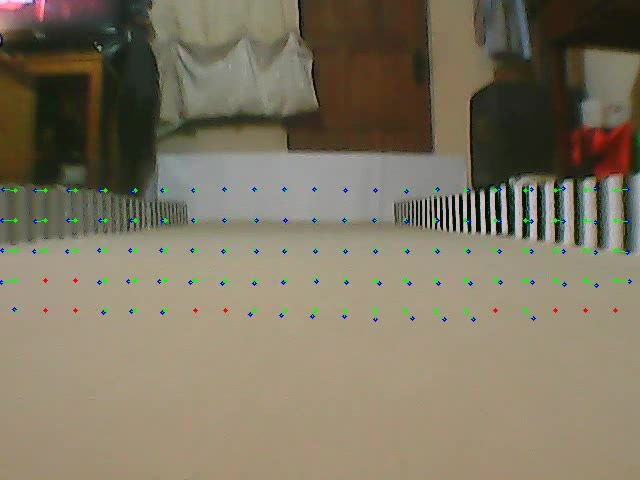
\includegraphics[width = 400pt]{images/travel_1.jpeg}
  \caption[Captura flujo óptico.]{Captura de flujo óptico desde el robot omidirecional.}
  \label{fig:travel_1}
\end{figure}

\begin{figure}[H]
  \centering
  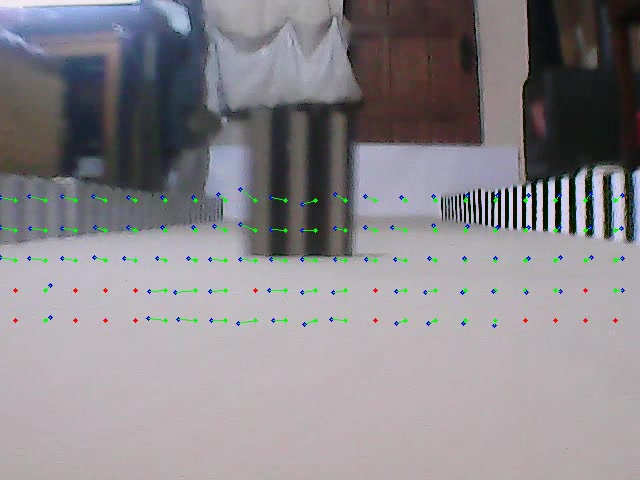
\includegraphics[width = 400pt]{images/travel_2.jpeg}
  \caption[Captura flujo óptico frente a obstaculo.]{Captura de flujo óptico del imagenes desde el robot omidirecional, frente a un obstaculo.}
  \label{fig:travel_2}
\end{figure}

El plano de la cámara está ubicado perpendicularmente al del desplazamiento del robot, por lo que solo se entrega a la red neuronal el flujo óptico que es calculado en el eje $X$ de la imagen, es decir, la cuantificación del desplazamiento lateral de los pixeles en la imagen.\\

Por cada \emph{frame} en el que se calcula el flujo óptico se obtiene un arreglo con un tamaño de 105 elementos que proporciona el desplazamiento de los puntos con respecto a la matriz antes descrita. Además del desplazamiento que tuvo el robot sobre el eje $X$ de la pista, en la figura \ref{fig:optical_flow} se muestra un ejemplo de esto. Esta es la información que posteriormente se le entrega a la red neuronal.\\

\begin{figure}[H]
\centering
\begin{verbatim}
	[15.1345, 45.7654, 75.4358,... 615.5472, 645.8256, 675.1234], [0.75]
\end{verbatim}
\caption[Captura del flujo óptico de un \emph{frame}.]{Ejemplo del flujo óptico obtenido de un \emph{frame} más el desplazamiento del robot.}
  \label{fig:optical_flow}
\end{figure}

El algoritmo \ref{DataCapture} muestra el pseudocodigo de como se realiza la captura del flujo óptico.\\

\begin{algorithm}[H]
\caption{Captura de datos}\label{DataCapture}
\begin{algorithmic}[1]
\Function{DataCapture}{}
\State $data\_input \gets [\,]$
\State $data\_output \gets [\,]$
\State $data\_mouse \gets [\,]$
\While{video\_capture}
\State $optical\_flow\_calc \gets calcOpticalFlow()$ 
\State $optical\_flow\_data \gets getXComponent(optical\_flow\_calc)$ \Comment Obtiene el compoenete $X$ del flujo óptico
\State $x,\, y \gets getMovement()$ \Comment Obtiene el desplazamiento del robot
\State $data\_input.append(optical\_flow\_data)$
\State $data\_output.append(normalize(x))$
\State $data\_mouse.append([x,\, y])$
\EndWhile

\State $saveData(data\_input,\, data\_output,\, data\_mouse)$
\EndFunction
\end{algorithmic}
\end{algorithm}

La información obtenida de cada \emph{frame} es almacenada en tres arreglos distintos: para el flujo óptico, el movimiento normalizado del robot en el eje $X$ y la información completa del movimiento tanto en el eje $X$ como en el $Y$. Cuando termina la captura de video se almacenan los tres arreglos en un archivo serializado. Por cada recorrido del robot por la pista se tiene una captura continua de video, entonces también se tiene un archivo con el flujo óptico y el desplazamiento realizado.\\

\section{Red neuronal}

La red neuronal es una adaptación de la implementada por \emph{Michael Nielsen} en del libro \emph{Neural Networks and Deep Learning} escrita en \emph{Python} \cite{NeuralNetworksAndDeepLearning} haciendo uso de la libreria \emph{numPy}, que contiene un paquete de funciones matemáticas para el trabajo con matrices multidimensionales \cite{numpy}, está tiene la finalidad de recibir la información visual obtenida por el cálculo del flujo óptico y direccionar correctamente el robot por la pista. Aquí se documenta el funcionamiento de la red y el método que se utiliza para hacer que esta aprenda.\\

\subsection{Funcionamiento}
 
Para representar la estructura de la red, la que cuenta con \emph{weights} y \emph{biases} (pesos y sesgos) por cada neurona, se utiliza un arreglo multidimensional por cada parámetro. Para los sesgos se utiliza una matriz de dos dimensiones, así obtenemos $b_{ij}$ que representa el sesgo para la $j$-$\acute{e}sima$ neurona en la $i$-$\acute{e}sima$ capa. La representación de los pesos se hace con una matriz de tres dimensiones, dando $w_{ijk}$ que se traduce como el peso de la $j$-$\acute{e}sima$ neurona de la $i$-$\acute{e}sima$ capa con la $k$-$\acute{e}sima$ neurona de la $i$+$1$-$\acute{e}sima$ capa.\\
 
La obtención de la salida de red neuronal, también llamado \emph{feedforward}, se hace ejecutando para cada capa la siguiente función:\\

\begin{equation}
	\begin{split}
	a' = \sigma{(z)}\\
	\end{split}
\end{equation}\\

donde $z$:\\

\begin{equation}
	\begin{split}
	z = (wa + b)\\
	\end{split}
\end{equation}\\

Si aplicamos la función $\sigma$ a la $i$-$\acute{e}sima$ capa usamos la función sigmoide $\sigma$ en cada elemento del arreglo $z$, $z$ contiene el resultado del producto punto entre los pesos y el arreglo $a$ más el sesgo de cada neurona. Donde $a$ es la salida de la $i$-$1$-$\acute{e}sima$ capa o si es la primera la entrada de la red. Dando como resultado la salida $a'$ la cual es el resultado $i$-$\acute{e}sima$ capa. El pseudocódigo se muestra en el algoritmo \ref{feedforward}.\\

\begin{algorithm}[H]
\caption{Red neuronal}\label{feedforward}
\begin{algorithmic}[1]
\Function{feedforward}{a}

\For{$b,\, w \gets biases,\, weights$ }
	\State $a \gets \sigma((w \cdot a)+b)$
\EndFor

\State \textbf{return} $a$
\EndFunction
\end{algorithmic}
\end{algorithm}

La implementación del algoritmo de \emph{backpropagation} consta de realizar el proceso de \emph{feedforward} para una determinada entrada y poder calcular con su salida esperada $y$ la siguiente ecuación de error:\\

\begin{equation}
	\begin{split}
	\delta^L = (a^L-y) \odot \sigma'(z^L)
	\end{split}
\end{equation}\\

Donde $a^{L}$ y $z^{L}$ pertenecen a la última capa $L$, el arreglo $\delta^{L}$ representa la influencia de la salida de la red en la funcion de costo. Ahora se obtiene la difencia de los sesgos y pesos de la capa $L$:

\begin{equation}
	\begin{split}
	b^L & = \delta^L\\
	w^L & = \delta^L \sigma(z^L)^t
	\end{split}
\end{equation}\\

Este procedimiento se propaga hacia atrás en la red por las capas $L-1, L-2, L-3...$ hasta alcanzar la primera capa. Para luego actualizar los parametros de red aplicando las diferencias obtenidas bajo un coeficiente de aprendizaje, este determina cuanto se deben modificar los parametros existentes en la red con respecto a las diferencias obtenidas del algoritmo de \emph{backpropagation}.

%\subsection{Diseño de capas}

\subsection{Entrenamiento}

Para entrenar la red neuronal se utiliza como entrada el flujo óptico obtenido de la captura de video de la pista de pruebas y como salida esperada la dirección en la cual se mueve el robot sobre el eje $X$ de la pista. Para modificar los parametros al interior de la red (pesos y sesgos), que se traduce como el aprendizaje de la red, se utiliza la técnica de \emph{backpropagation}, véase sección \ref{redes_neuronales}.\\

La implementación de red reorganiza de forma aleatoria los datos de entrenamiento e itera el entrenamiento un número determinado de veces. Al final de cada iteración se valida el entrenamiento con los datos de prueba, así se evalúa el transcurso del entrenamiento. Al finalizar la iteracion se guarda la red que tuvo un mejor desempeño en la validacion del entrenamiento.\\

La generación de set de datos del cual la red aprende se hace por medio de un esquema \emph{on-the-fly} \cite{pomerleau1989alvinn}, el cual tiene como objetivo que la red neuronal imite el comportamiento de un humano al realizar la misma tarea, la cual es desplazar el robot por la pista de pruebas. Por lo que el flujo óptico y la dirección del robot se obtiene de la conducción manual del robot.\\

La salida esperada de la red neuronal, que representa la direccion en la cual debe moverse el robot mientras se desplaza por la pista y que es utilizada como parámetro en el entrenamiento por \emph{backpropagation}, es obtenida por el seguimiento de los movimientos que realice el robot por medio de un sensor óptico de movimiento. La arquitectura de la red neuronal tendrá una sola salida la que estará normalizada entre cero y uno, por lo que la dirección del robot será representada por un solo valor.\\

Se realizan dos entrenamientos: el primero con los datos obtenidos del robot al desplazarse sin obstáculos, el segundo utiliza los mismos datos y se le suman los datos de los recorridos con obstáculos. Son usadas dos redes neuronales, cada red neuronal tiene 105 entradas y una sola salida, la primera solo tiene la una capa oculta de 50 neuronas mientras que la segunda cuatro capas ocultas con 100, 70, 40 y 10 neuronas respectivamente. En cada entrenamiento consta de 30 iteraciones y un coeficiente de entrenamiento de 0.5. En la tabla \ref{tab:training validation data} se muestra el número de datos utilizados para cada etapa del entrenamiento. El algoritmo \ref{alg:training} muestra el pseudocódigo del entrenamiento.\\

\begin{table}[H]
\caption[Datos de entrenamiento y validación]{Datos de entrenamiento y validación}
\makebox[\textwidth][c]{	
	\fontfamily{cmss}\selectfont{
	\begin{tabular}{c|cc}
	\addlinespace
	\toprule
	{\bf } & \multicolumn{ 2}{c}{{\bf Datos de entrenamiento}} \\
	\midrule
	{\bf Etapa} & {\bf Entrenamiento} & {\bf Validación} \\
	1  & 34755 & 7367 \\
	2  & 66297 & 20635 \\
	\bottomrule
	\end{tabular}
	}
}
\label{tab:training validation data}
\end{table}

\begin{algorithm}[H]
\caption{Entrenamiento}\label{alg:training}
\begin{algorithmic}[1]
\Function{Training}{$training\_data,\, test\_data,\, epoch,\, eta$}
\State $result \gets [\,]$
\For{$epoch$}
\State $training\_data \gets shuffle(training\_data)$

\For{$x,\, y \gets training\_data$}
	\State $backpropagation(x,\, y,\, eta)$
\EndFor

\State $effectiveness,\, mse = evaluate(test\_data)$
\State $result.append([effectiveness,\, mse])$
\EndFor

\State \textbf{return} $result$
\EndFunction
\end{algorithmic}
\end{algorithm}

\section{Conducción autónoma}

El objetivo principal es conseguir la conducción autónoma del robot y que este sea capaz de evadir los obstáculos que se dispongan en la pista de pruebas. Para lograr esto es necesario utilizar la captura de video en tiempo real para calcular el flujo óptico, una vez obtenido se entregado a la red neuronal. Una vez que la red neuronal entrega el resultado este es utilizado para dirigir el robot, para volver a repetir el proceso en el siguiente \emph{frame} de la captura de video.\\

La captura de video consiste en obtener los \emph{frame} que envía la cámara digital, para posteriormente calcular el flujo óptico por cada uno de estos. Una vez que se tiene el flujo óptico a este se le obtiene su componente en eje $X$ y es entregado a la red neuronal.\\

La red realiza el proceso de \emph{feedforward} y el valor entregado, que está normalizado entre cero y uno, corresponde a la dirección a la cual debe moverse el robot. La información que recibe el robot tiene un rango entre 1000 y 2000, por lo que antes de ser enviada debe ser normaliza dentro de estos valores.\\

Después de enviar los datos al robot se leen los provenientes del sensor de movimiento, los cuales son almacenados para tener un registro des los movimientos realizados por el robot al realizar la conducción autónoma.\\

Una vez terminado el procedimiento se obtiene el nuevo \emph{frame} de la cámara de video y se repite el proceso mencionado, el algoritmo \ref{alg:AutoDriving} muestra el pseudocódigo de la conducción autónoma.\\

\begin{algorithm}[H]
\caption{Conducción autónoma}\label{alg:AutoDriving}
\begin{algorithmic}[1]
\Function{AutoDriving}{}
\State $data\_mouse \gets [\,]$
\While{video\_capture}
\State $optical\_flow\_calc \gets calcOpticalFlow()$ 
\State $optical\_flow\_data \gets getXComponent(optical\_flow\_calc)$ \Comment Obtiene el compoenete $X$ del flujo óptico
\State $net\_output \gets net.feedforward(optical\_flow\_data)$
\State $move\_data \gets normalize(nte\_output)$
\State $writeData(move\_data)$ \Comment Envia los datos al robot para realizar el movimiento correspodiente
\State $x,\, y \gets getMovement()$ \Comment Obtiene el desplazamiento del robot
\State $data\_mouse.append([x,\, y])$
\EndWhile

\State $saveData(data\_mouse)$
\EndFunction
\end{algorithmic}
\end{algorithm}

\section{Procesamiento de datos}

Todo el procesamiento de datos es realizado por un computador externo al robot, las tareas que este realiza son: la captura de datos, entrenamiento de red neuronal y conducción autónoma. Para esto se utiliza el lenguaje de programación \emph{Python} en su versión 2.7.\\

El computador utilizado es un notebook \emph{ProBook} 4440s con las siguientes característica:

\begin{itemize}
    \item {\bf Procesador:} Intel Celeron(R) CPU B840  1.90GHz x 2
    \item {\bf Memoria:} 4 GB
    \item {\bf Sistema Operativo:} Debian GNU/Linux 8 (jessie)
    \item {\bf Arquitectura: } 64-bit
\end{itemize}

Los periféricos utilizados son conectados por medio de puerto USB, el robot cuenta con un \emph{hub} donde esta conectada la cámara digital, el sensor de movimiento y el Arduino UNO, por lo que al computador solo llega una interfaz USB.\\

Para obtener los datos del sensor de movimiento se programó un \emph{thread} que está constantemente leyendo el archivo \texttt{/dev/input/mice} el cual entrega el dato \emph{raw} (en bruto) del movimiento del sensor. Para comunicar el Arduino UNO también se utiliza un \emph{thread} que establece comunicación serial  que está configurada a 57600 \emph{baudios}.\\

\section{Robot omnidireccional}

El diseño del robot está basado en uno del repositorio de diseños 3D thingiverse (https://www.thingiverse.com/thing:167923), de este se tomó el concepto de las ruedas omnidireccionales las que se rediseñaron para este robot en especifico.\\

\subsection{Diseño del robot}

El diseño del robot contempla el uso de 4 ruedas omnidireccionales, las que se sitúan de forma perpendicular alrededor del robot, cada rueda esta separada una de la otra por 90$^{\circ}$. La construcción de cada rueda consta de dos ruedas paralelas rotadas sobre el eje de giro 45$^{\circ}$ una de la otra, unidas por medio de tres tornillos. Cada una de estas ruedas cuenta a su vez con cuatro ruedas o rodillos en su circunferencia colocadas perpendicularmente separadas cada una por 90$^{\circ}$, esto permite tener un solapamiento con los rodillos de la otra rueda ubicada paralela a esta. Los rodillos van fijos a un eje de 2mm que los atraviesa y puede girar libremente en el soporte de la rueda. Cada rueda tiene un diámetro de 80mm y un ancho de 40mm, en la figura \ref{fig:image_omni_whell_2} se puede ver la construcción de esta.\\

\begin{figure}[H]
  \centering
  \includesvg[width = 200pt, svgpath = images/image_omni_whell_2]{}
  \caption[Rueda omnidireccional.]{Diseño de rueda omnidireccional.}
  \label{fig:image_omni_whell_2}
\end{figure}

Cada rueda cuenta con un acople, que en un extremo va atornillado a la rueda por tres tornillos y en el otro va sujeto a presión al eje de la caja reductora del motor, como muestra la figura \ref{fig:cupling}.\\

\begin{figure}[H]
  \centering
  \includesvg[width = 200pt, svgpath = images/Coupling]{}
  \caption[Acople entre la rueda y la caja reductora.]{Acople para unir las ruedas del robot con la caja reductora de los motores.}
  \label{fig:cupling}
\end{figure}

A su vez los motores y su respectiva caja reductora están unidos por una extensión que permite unirlos al cuerpo principal, de esta forma se puede modificar el diámetro total del robot sin tener que modificar también el cuerpo principal, \ref{fig:arm}\\

\begin{figure}[H]
  \centering
  \includesvg[width = 200pt, svgpath = images/arm]{}
  \caption[Extensión para unir los motores.]{Extensión para unir los motores.}
  \label{fig:arm}
\end{figure}

En el cuerpo principal se posicionan el resto de los componentes necesarios para el funcionamiento, estos son el microcontrolador, los \emph{driver} para los motores, las baterías, el receptor de radio, la cámara digital y sensor de movimiento. El cuerpo fue diseñado de acuerdo a las dimensiones de cada componente, de esta manera se pueden colocar de manera precisa, además de usar las fijaciones para las cuales fueron diseñados, que se muestra en la figura \ref{fig:frame}.\\

\begin{figure}[H]
  \centering
  \includesvg[width = 300pt, svgpath = images/frame]{}
  \caption[Cuerpo principal robot omnidireccional.]{Cuerpo principal donde se alojan todos los componentes del robot omnidireccional.}
  \label{fig:frame}
\end{figure}

El compartimiento para las baterías es ubicado debajo de cuerpo principal, este permite la fijación de baterías de litio estándar 18650 colocadas en serie, permite colocar un total de 3 baterías. El diseño se puede ver en la figura \ref{fig:battery_compartment}.

\begin{figure}[H]
  \centering
  \includesvg[width = 300pt, svgpath = images/battery_compartment]{}
  \caption[Compartimiento de baterías.]{Compartimiento para colocar en serie las tres baterías de litio 18650.}
  \label{fig:battery_compartment}
\end{figure}

Debajo de este, en contacto con la superficie donde se desplaza el robot, va el soporte del sensor óptico de movimiento. En la figura \ref{fig:mouse_holder} se puede ver que el soporte cuenta con perforaciones por las que se atornilla al cuerpo principal por medio de separadores, para ajustar la altura del soporte para que quede posicionado de forma precisa sobre la superficie.\\

\begin{figure}[H]
  \centering
  \includesvg[width = 300pt, svgpath = images/mouse_holder]{}
  \caption[Soporte sensor óptico.]{Soporte para la instalación del sensor óptico que registra las trayectorias realizadas por el robot.}
  \label{fig:mouse_holder}
\end{figure}

Al frente del robot va instalada la cámara digital, esta va sobre un soporte que se ajusta a sus dimensiones, el que a su vez va unido al cuerpo principal, en la figura \ref{fig:camera_holder} se muestra el diseño, que incluye una ranura para posicionar el cable de la cámara.\\

\begin{figure}[H]
  \centering
  \includesvg[width = 300pt, svgpath = images/camera_holder]{}
  \caption[Soporte cámara digital.]{Soporte sobre el cual va la cámara digital.}
  \label{fig:camera_holder}
\end{figure}

El ensamble completo con todos los componentes diseñados para la construcción del robot se puede ver en la figura \ref{fig:robot_assembly}. Todos los acoples mecánicos fueron realizados con tornillos de métrica 3 (M3), cortados una medida específica para cada unión.

\begin{figure}[H]
  \centering
  \includesvg[width = 400pt, svgpath = images/robot_assembly]{}
  \caption[Ensamble robot omnidireccional.]{Ensamble completo del robot omnidireccional.}
  \label{fig:robot_assembly}
\end{figure}

\begin{figure}[H]
  \centering
  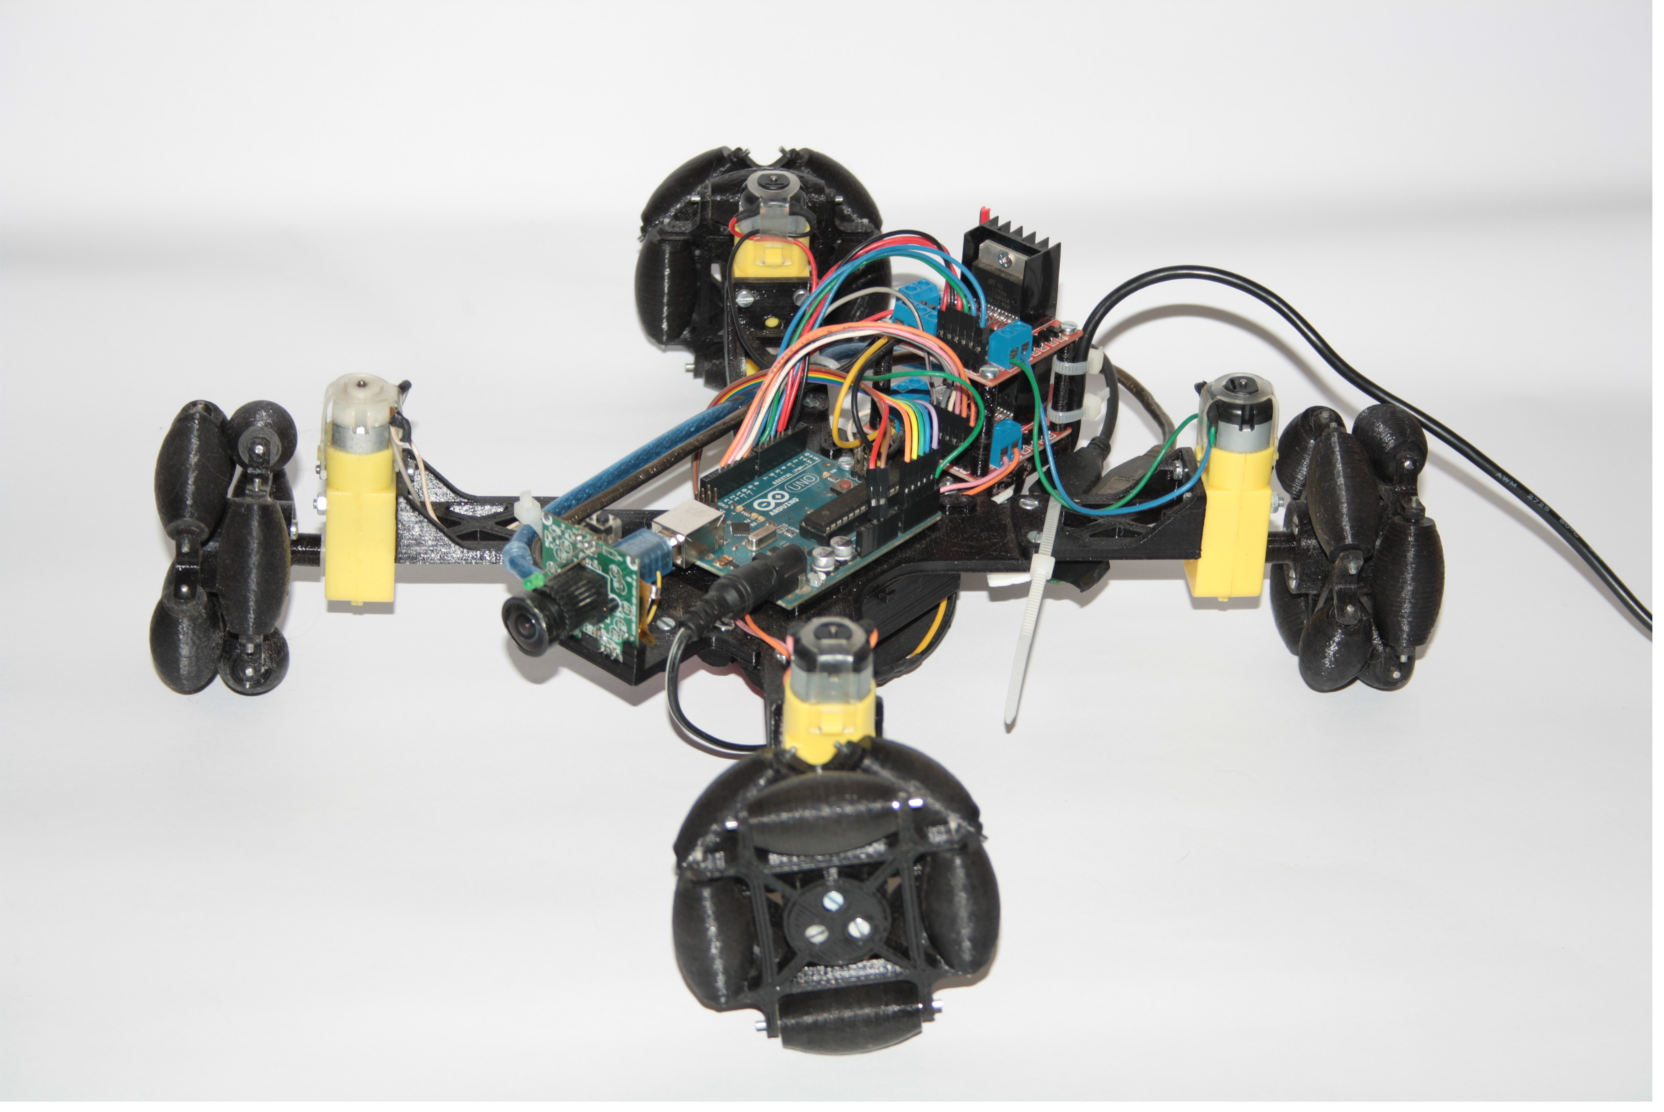
\includegraphics[width = 400pt]{robot.png}
  \caption[Robot omnidireccional completo.]{Robot completo con todos los componentes.}
  \label{fig:robot}
\end{figure}

Los componentes mencionados y diseñados específicamente para el robot (ruedas omnidireccionales, extensiones para los motores, cuerpo principal, compartimiento para baterías, soporte para la cámara digital y soporte para el sensor óptico) fueron diseñados con la herramienta FreeCAD, un modelador 3D parametrico. Para el proceso de fabricación se utiliza Sli3r, que comvierte los modelos 3D a instrucciones para la impresora 3D. Las piezas son construidas con impresión 3D de filamento fundido (FFF del termino en inglés: \emph{Fused Filament Fabrication}) con las siguientes especificaciones:\\

\begin{itemize}
	\item {\bf Material:} PLA 1.75mm
	\item {\bf Diametro boquilla:} 0.4mm
	\item {\bf Altura de capa:} 0.2mm
	\item {\bf Temperatura de boquilla:} 220$^{\circ}$
	\item {\bf Temperatura placa:} 60$^{\circ}$
	\item {\bf Velocidad impresion:} 30mm/s
	\item {\bf Velocidad recorrido:} 60mm/s
	\item {\bf Relleno:} 15\%
	\item {\bf Patron relleno:} rectilíneo
\end{itemize}

La especificación completa de la configuracion de la impresora se puede ver en el anexo \ref{appendix:3D printer setting}

\subsection{Control de las ruedas}

El desplazamiento del robot es producido por cuatro motores, estos no van en conexión directa con las ruedas, si no que por medio de una caja reductora y esta transmite el movimiento del motor a las ruedas. Los motores son de tamaño estándar 130 alimentados con 12v de corriente continua (DC) con una caja reductora TT a 90$^{\circ}$, de relación 120:1, como se muestra en la figura \ref{fig:motor}.\\

\begin{figure}[H]
  \centering
  \includesvg[width = 100pt, svgpath = images/motor]{}
  \caption[Motor con caja reductora del robot omnidireccional.]{Motor con caja reductora del robot omnidireccional.}
  \label{fig:motor}
\end{figure}

Los motores son controlados por el \emph{driver} (controlador) L298N, este cuenta con dos puentes H, uno por motor, por lo que el robot utiliza dos controladores. Los controladores son alimentados con 12v y estos son los que suministran la energía a los motores.\\

La fuente de energía del robot es proporcionada por baterías de litio, se utilizan tres de estandar 18650 conectadas en serie, cada batería es de 3,7v, por lo que en total en conjunto se tiene un voltaje nominal de 11.1v, con las baterías cargadas al 100\% de su capacidad su voltaje es de 12,6v.\\

Los movimientos del robot son realizados posteriormente al cálculo de las velocidades y dirección de giro de cada rueda, esta tarea es realizada por el microcontrolador, el utilizado es un ATmega328P bajo la infraestructura de Arduino UNO. El microcontrolador toma como entrada la velocidad y dirección a la cual debe moverse y realiza los cálculos para obtener los valores asociados a cada motor. Las salidas de control van dirigidas a los controladores de los motores, se utilizan tres líneas por cada motor, figura \ref{fig:ATmega328P_L298N}, dos para controlar la dirección del motor y la tercera para la velocidad, por lo que se tiene un total de doce salidas de control para todos los motores.\\

\begin{figure}[H]
  \centering
  \fontfamily{cmss}\selectfont{
  \includesvg[width = 400pt, svgpath = images/ATmega328_L298]{}
  }
  \caption[Control de de los motores.]{Control del microcontrolador ATmega328P sobre uno de los motores, por medio del controlador L298N.}
  \label{fig:ATmega328P_L298N}
\end{figure}

El control sobre los motores se hace de la siguiente manera: En el controlador L298N las salidas reflejan el estado en el que se encuentran las entradas, por lo que OUT1 tendrá el mismo estado que In1, lo mismo sucede cuando con OUT2 y In2, siempre y cuando En este en estado lógico alto. La tabla \ref{tab:l298 in out} muestra el comportamiento del controlador con respecto a las distintas entradas.\\

\begin{table}[H]
\caption[Comportamiento de las salidas del controlador L298.]{Comportamiento de las salidas del controlador L298N. L = estado lógico bajo, H = estado lógico alto y X = cualquier estado.}
\centering
	\fontfamily{cmss}\selectfont{
	\begin{tabular}{|c|c|c||c|c|}

		\hline
			\multicolumn{3}{|c||}{Entradas} & \multicolumn{2}{c|}{Salidas}\\
		\hline
			In1 = H & In2 = L & En = H & OUT1 = H & OUT2 = L\\
		\hline
			In1 = L & In2 = H & En = H & OUT1 = L & OUT2 = H\\
		\hline
			In1 = X & In2 = X & En = L & OUT1 = L & OUT2 = L\\
		\hline
	\end{tabular}
	}

\label{tab:l298 in out}
\end{table}

De esta forma variando el estado de las entradas es posible cambiar la dirección hacia donde giran los motores, ahora para establecer la velocidad a los motores se utiliza la tercera entrada En con una señal \emph{PWM} (sigla del inglés: \emph{Pulse-width modulation}) que mediante la variación del \emph{duty cycle} (ciclo de trabajo) logra establecer la variación de la velocidad. El ciclo de trabajo se define como el tiempo en que la señal se encuentra en estado alto, por ejemplo, en un ciclo de trabajo del 50\% la mitad del tiempo la señal está en alto y la otra mitad en bajo, en un ciclo del 25\% la señal está en alto solo el 25\% y el 75\% restante del tiempo está en estado bajo \cite{barrett2006microcontrollers}, como muestra la figura \ref{fig:pwm}.\\

\begin{figure}[H]
  \centering
  \fontfamily{cmss}\selectfont{
  \includesvg[width = 300pt, svgpath = images/pwm]{}
  }
  \caption[Ciclo de trabajo de señal \emph{PWM}]{Señal \emph{PWM} con distintos ciclos de trabajo.}
  \label{fig:pwm}
\end{figure}
 
Esta señal de control es producida por el microcontrolador a una frecuencia de 490 Hz, con una resolución de 8 bit, es decir, el ciclo de trabajo puede ser configurado con un rango de valores entre 0 y 255, siendo 0 un ciclo de trabajo del 0\% y 255 del 100\% \cite{referenceAnalogWrite}.\\

\subsection{Enlace de radio}

Para dar al robot su dirección y velocidad se utiliza un enlace de radio 2.4GHz el que proporciona hasta seis canales de comunicación, para el control de robot solo se utilizan dos. Cada canal se lee desde el receptor de radio por separado por el microcontrolador, utilizando una entrada por canal. La señal se codifica mediante \emph{PWM} donde la duración del pulso determina el valor del canal, cada pulso se produce en serie uno tras otro, este valor va en el rango de 1000$\mu$s a 2000$\mu$s.\\

\begin{figure}[H]
  \centering
  \fontfamily{cmss}\selectfont{
  \includesvg[width = 300pt, svgpath = images/pwm_radio]{}
  }
  \caption[Señal \emph{PWM} de los canales de radio.]{Señal \emph{PWM} de distintos canales, el pulso tiene una tiempo de duracion minimo de 1000$\mu$s y máximo de 2000$\mu$s.}
  \label{fig:pwm}
\end{figure}

Para obtener el valor de cada canal desde el receptor con el microcontrolador se lee la señal de un canal y se toma el tiempo, en milisegundos, que esta señal permanece con un valor alto, el tiempo registrado corresponderá al valor de dicho canal, esto se repite para el resto de los canales.\\
 
Los canales utilizados corresponden a uno y dos (ch1 y ch2), de estos se normalizan sus valores a un rango entre -500 y 500, con estos se conforma un vector $\vec{d}$ con coordenadas (ch1, ch2), como muetsra la figura \ref{fig:radio_values}, con este vector se calcula posteriormente el movimiento del robot.\\

\begin{figure}[H]
  \centering
  \fontfamily{cmss}\selectfont{
  \includesvg[width = 300pt, svgpath = images/radio_values]{}
  }
  \caption[Vector formado por las entradas de radio]{Vector formado por los valores de los canales uno y dos obtenidos desde el receptor de radio.}
  \label{fig:radio_values}
\end{figure}

\subsection{Movimiento}

Primero se necesita establecer un marco de referencia, el robot es capaz de desplazarse en dos dimensiones sobre un plano, este está formado por los ejes $X$ e $Y$. Cuando se menciona que el robot se mueve hacia adelante hace su recorrido avanzando sobre el eje $Y$, al contrario, cuando se mueve hacia atrás retrocede en el eje $Y$, como esta reprecentado en la figura \ref{fig:omni_direcition}. Ahora cuando se mueve a la derecha, avanza en el eje $X$ y a la izquierda retrocede. Haciendo una comparación con los cuadricópteros, el movimiento hacia adelate y atrás del robot corresponde al movimiento de \emph{pich} en el cuadricóptero y los de derecha e izquierda al \emph{roll}. No está dentro de los alcances contemplar el movimiento de \emph{yaw}.\\

\begin{figure}[H]
  \centering
  \fontfamily{cmss}\selectfont{
  \includesvg[width = 250pt, svgpath = images/omni_direction]{}
  }
  \caption[Desplazamiento del robot sobre el plano $XY$.]{Desplazamiento del robot sobre el plano conformado por los ejes $X$ e $Y$.}
  \label{fig:omni_direcition}
\end{figure}

El movimiento del robot está determinado por dos parámetros, hacia donde debe moverse y a que velocidad. Con esto se tiene un vector, que llamaremos $\vec{d}$, donde la dirección de este es la misma que debe seguir el robot y la magnitud es la velocidad del movimiento. Dado que las ruedas del robot están dirigidas en distintas orientaciones no es posible moverse directamente en la dirección de $\vec{d}$. Cada rueda se mueve en una dirección distinta con su propio vector de movimiento, por lo que para poder desplazarse en $\vec{d}$ se tiene que realizar la suma de los vectores de cada rueda, de tal forma que el resultado coincida con $\vec{d}$.\\

Si bien el robot cuenta con cuatro ruedas, con los movimientos que se tiene contemplados hacer (delante, atrás, derecha e izquierda) siempre un par de ruedas se mueven en paralelo, como muestra la figura \ref{fig:omni_vector}, así los movimientos de robot pueden descomponerse en dos vectores: $\vec{r_{1}}$ y $\vec{r_{2}}$, la magnitud de estos representa la velocidad a la que gira cada rueda. La suma de estos debe dar $\vec{d}$, como muestra la figura \ref{fig:vec_sum}.\\

\begin{figure}[H]
  \centering
  \begin{large}
  \includesvg[width = 200pt, svgpath = images/omni_vector]{}
  \end{large}
  \caption[Movimiento de las ruedas del robot omnidireccional.]{$\vec{r_{1}}$ y $\vec{r_{2}}$ pares de ruedas que se mueven de forma paralela.}
  \label{fig:omni_vector}
\end{figure}

\begin{figure}[H]
  \centering
  \begin{large}
  \includesvg[width = 200pt, svgpath = images/vec_sum]{}
  \end{large}
  \caption[Suma de los vectores que dan la dirección del robot.]{Suma de los vectores $\vec{r_{1}}$ y $\vec{r_{2}}$ que dan como resultado la dirección del robot.}
  \label{fig:vec_sum}
\end{figure}

Para realizar esta suma primero se obtienen las proyecciones de $\vec{d}$ sobre el eje $X$ e $Y$, dando como resultado $\vec{d_{x}}$ y $\vec{d_{y}}$. El ángulo $\theta$ se mide entre el $\vec{d}$ y el eje $X$ como muestra la figura \ref{fig:vec_proyection}.\\

\begin{equation}
	\begin{split}
	\vec{d_{x}} & = \lvert \vec{d} \rvert \cos(\theta)\\
	\vec{d_{y}} & = \lvert \vec{d} \rvert \sin(\theta)\\
	\end{split}
\end{equation}\\

\begin{figure}[H]
  \centering
  \begin{large}
  \includesvg[width = 200pt, svgpath = images/vec_proyection]{}
  \end{large}
  \caption[Proyección del vector $\vec{d}$ sobre el eje $X$ e $Y$.]{Proyección del vector $\vec{d}$ sobre el eje $X$ e $Y$, dando los vectores $\vec{d_{x}}$ y $\vec{d_{y}}$ .}
  \label{fig:vec_proyection}
\end{figure}

Ahora la magnitud de $\vec{r_{1}}$ y $\vec{r_{2}}$ se puede definir como:\\

\begin{equation}
	\begin{split}
	\vec{r_{1}} & = \vec{d_{x}}\cos(\pi/4)  + \vec{d_{y}}\cos(\pi/4)\\
	\vec{r_{2}} & = -\vec{d_{x}}\cos(\pi/4) + \vec{d_{y}}\cos(\pi/4)\\
	\end{split}
\end{equation}\\

Donde $\pi/4$ es ángulo de $\vec{r_{1}}$ y $\vec{r_{2}}$ sobre el eje $X$. Si la magnitud de los vectores toma un valor negativo es debe invertir la dirección de las ruedas.\\

En este capítulo fueron descrito todo lo que se necesita implementar para poder llegar a dar con la solución. Se detalló la forma en cómo se obtiene el flujo óptico y se utiliza para generar los datos necesarios, También se explica la utilización de la red neuronal y la forma en que va a ser entrenada, Por último se mostró el diseño de cada componente necesario para construir el robot omnidireccional y como este logra desplazarse.\\

\chapter{Pruebas}

Las pruebas que se realizan para comprobar si la red neuronal aprende y es capaz de evadir obstáculos se dividen en dos etapas: La primera consta en mover el robot sobre la pista de pruebas sin colocar obstáculos, sólo con información visual a los costados, la que será captada como flujo óptico, esta permitirá que el robot evite los bordes de la pista y sea capaz de centrarse dentro de esta. En la segunda etapa se mantendrá el mismo esquema de la primera, además de incluir un obstáculo en la pista de pruebas, que el robot tendrá que evadir.\\

\section{Comprobación de aprendizaje}

Por cada una de las etapas se comprobará de dos formas distintas si la red neuronal está aprendiendo. La primera es evaluando el aprendizaje con un set de datos de prueba, que no fue usado para el entrenamiento, aquí se evalúa cuánto difiere la salida teórica que debería entregar la red, salida esperada, con la que entrega realmente la red. Esta diferencia se considera \emph{test error} (error de prueba) y esta será obtenida por la técnica de \emph{Validation Set Approach} (enfoque de conjunto de validación) la que consiste en dejar parte del conjunto de entrenamiento para validar cuán efectivo fue este \cite{james2014introduction}.\\

Para la primera etapa se usaron 34755 datos para el entrenamiento y 7367 para la validación, en la segunda etapa se suman a los datos ya utilizados 31542 datos de entrenamiento y 13268 de validación. Dando un total de datos para la segunda etapa de 66297 elementos para entrenamiento y 20635 para validación.\\
 
La cuantificación del error se mide de dos formas distintas: La primera es mediante es el error cuadrático medio \emph{MSE} (del ingles: \emph{mean squared error}):\\

\begin{equation}
	MSE = \frac{1}{n} \sum^n_{x=1} (y_i-a^L(x_i))^2
\end{equation}\\

Donde $y_i$ es la salida esperada y $a^L(x_i)$ es la salida que da la última capa $L$ de la red neuronal con la entrada $x_i$, con un set de prueba de tamaño $n$. En el segundo método se mide el porcentaje de efectividad de la red, cuantificando la cantidad de veces que la red entrega una salida que satisface a una respuesta esperada sobre el total de respuestas entregadas. Para saber si la salida cumple esta condición se establece un margen de aceptación de 90$\%$, donde la salida de la red no puede desviarse más allá de este porcentaje para que se considere salida correcta. El entrenamiento se considera exitoso si la eficacia de la red está sobre el 90$\%$.\\
 
La segunda comprobación de entrenamiento se realizará de forma empírica, comparando el comportamiento de la conducción manual del robot, contra la conducción autónoma guiada por la red neuronal, cada vez que el robot se desplace por la pista de pruebas se deja registro de su desplazamiento, por lo que se puede comparar el recorrido realizado de forma manual y el de forma autónoma.\\

% Para considerar la prueba exitosa la desviación de las dos trayectorias no debe ser mayor a [medida de desviación].\\
 
\section{Obtención de datos}
 
La obtención del conjunto datos, para realizar las pruebas, consta de conducir de forma manual el robot repetidas veces por la pista de pruebas, colocando el robot en posiciones definidas al comienzo de la pista y dirigirlo hasta un punto determinado de esta.\\
 
Para la primera etapa, sin importar la posición de inicio, tiene como objetivo mover el robot al centro de la pista direccionando sobre el eje $X$ mientras se desplaza por la pista en el eje $Y$, para que de esta forma la red neuronal pueda aprender a direccionar el robot evadiendo los bordes de la pista.\\
 
En la segunda etapa se posicionará un obstáculo dentro de la pista, al igual que en la primera etapa, también se deberá centrar el robot dentro de la pista, pero al enfrentarse a un obstáculo este debe ser evadido.\\

Para la recopilación de datos el recorrido del robot comienza en tres posiciones distintas en el inicio de la pista, las posiciones están a 20 cm del borde derecho, al centro y a 20 cm del borde izquierdo. Por cada una de estas se registran 30 recorridos del robot sobre la pista para los datos de entrenamiento y 10 para los datos de prueba. Obteniendo la información de flujo óptico y el recorrido hecho por este. El recorrido registrado es a una velocidad constante de 60 cm por segundo y una distancia de 2 mt desde el comienzo de la pista.\\
 
Para la recopilación de datos con obstáculos, se utilizará el mismo esquema anterior, pero se posiciona un obstáculo dentro de pista en distintas posiciones predefinidas. El obstáculo está construido con tres cilindros de cartón pintados de negro con una franja vertical blanca de 12 mm de ancho (para aumentar el flujo óptico registrado por el robot), cada cilindro tiene un diámetro de 5 cm y 18.5 cm de alto.\\

El obstáculo es posicionado en tres lugares distintos dentro de la pista, a 25 cm del borde derecho de la pista, al centro de la pista y a 25 cm del borde izquierdo, cada posición está a 1,5 mt del inicio de la pista.\\

Por cada posición del obstáculo se registran cinco recorridos para los datos de entrenamiento y tres para los da prueba por cada una de las tres posición de inicio, dando un total de quince recorridos para el entrenamiento y nueve para las pruebas por cada posición del obstáculo.\\
 
La construcción de la pista de pruebas necesita de un material que proporciona tracción a las ruedas del robot, por lo que se utiliza una alfombra de cubre pisos de 1 metro de ancho y 4 metros de largo, de color \emph{beige} para proporcionar mayor contraste frente a los obstáculos. Los bordes de la pista están construidos de poliestireno expandido de 1 cm de espesor, 25 cm de alto y cubren todo el recorrido de la pista de 4 mt, con un patrón regular líneas verticales de color blanco y negro de 5 cm de ancho.\\

En el reciente capítulo de detallo cómo son llevadas a cabo las pruebas, estas son las que daran a conocer si la red neuronal es capaz de aprender a mantenerse en la pista y evadir obstáculos. Se explicaron los procedimientos necesarios para llevar a cabo las pruebas, los mecanismos por los que se van a medir los resultados, además de especificar el escenario donde van a realizarse.\\

\chapter{Resultados}

A continuación se muestran los resultados obtenidos al realizar la comprobación del entrenamiento de la red neuronal y las pruebas empíricas de conducción autónoma del robot tanto para la primera etapa, que consta de evitar los bordes de la pista, como para segunda que tiene como objetivo evadir los obstáculos que se le presentan al robot.\\

\section{Entrenamiento de la red neuronal}

En este apartado se muestran los resultados obtenidos después de entrenar la red neuronal en los dos escenarios descritos en las pruebas: en la evasión de los bordes de la pista y la evasión de objetos.\\

\subsection{Evasión de bordes}

El entrenamiento de la red neuronal en esta etapa se hace con un set de 34755 datos y la validación con un set de 7367 datos. El entrenamiento consta de 30 iteraciones, es decir que la red se entrena por \emph{backpropagation} luego se calcula el \emph{test error} por medio de su efectividad y MSE, luego con red ya entrenada se repite el proceso por un total de 30 veces. El entrenamiento es realizado a dos redes distintas la primera con una sola capa oculta de 50 neuronas (denotada a continuación como Red.1.A), la segunda con 4 capas ocultas de 100, 70, 40, 10 neuronas respectivamente (denotada a continuación como Red.1.B). En la figura \ref{fig:net.1.a} y \ref{fig:net.1.b} se muestran los resultados obtenidos con las dos redes neuronales.\\


\begin{figure}
  \centering
  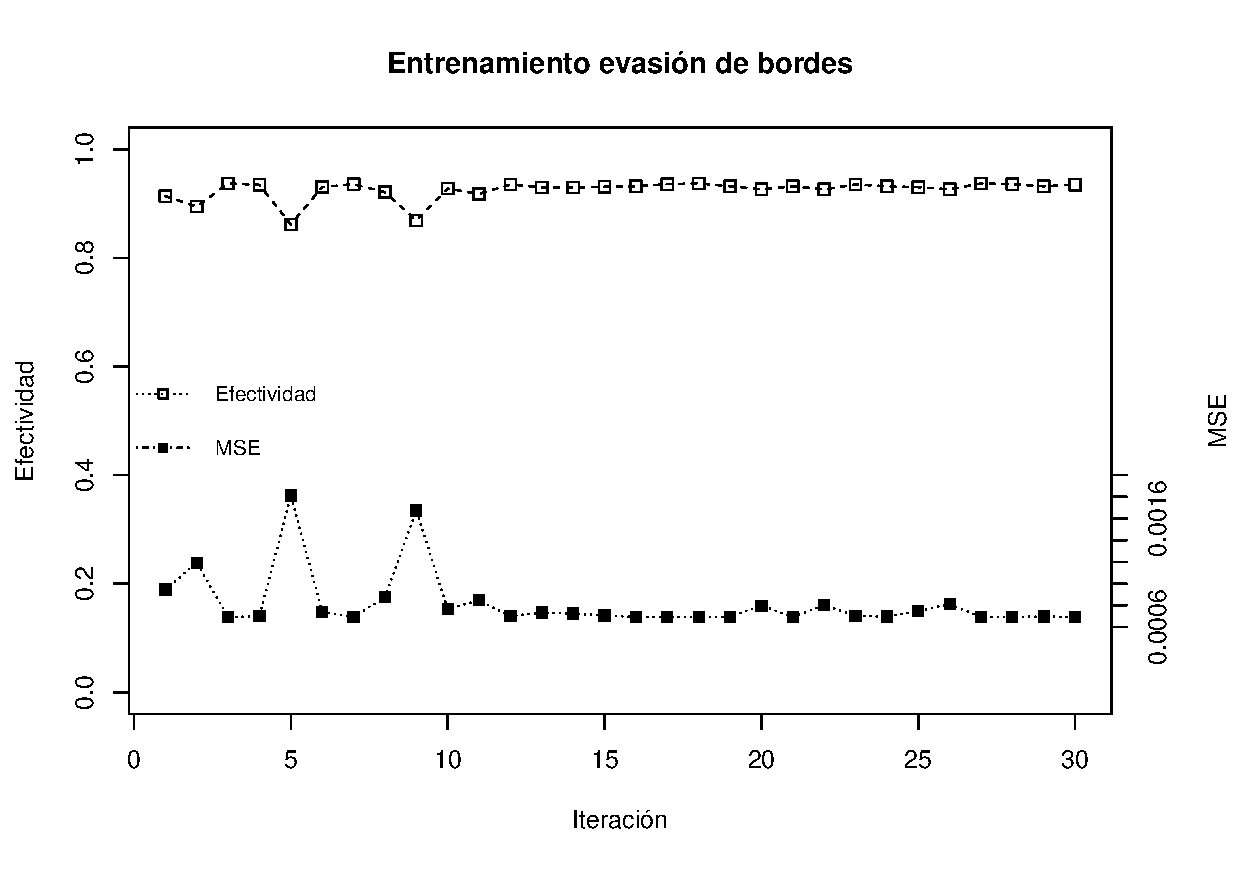
\includegraphics[width = 450pt]{images/plot_net_1_a.pdf}
  \caption[Entrenamiento primera etapa Red.1.A.]{Resultado del entrenamiento después de 30 iteraciones de Red.1.A.}
  \label{fig:net.1.a}
\end{figure}

\begin{figure}
  \centering
  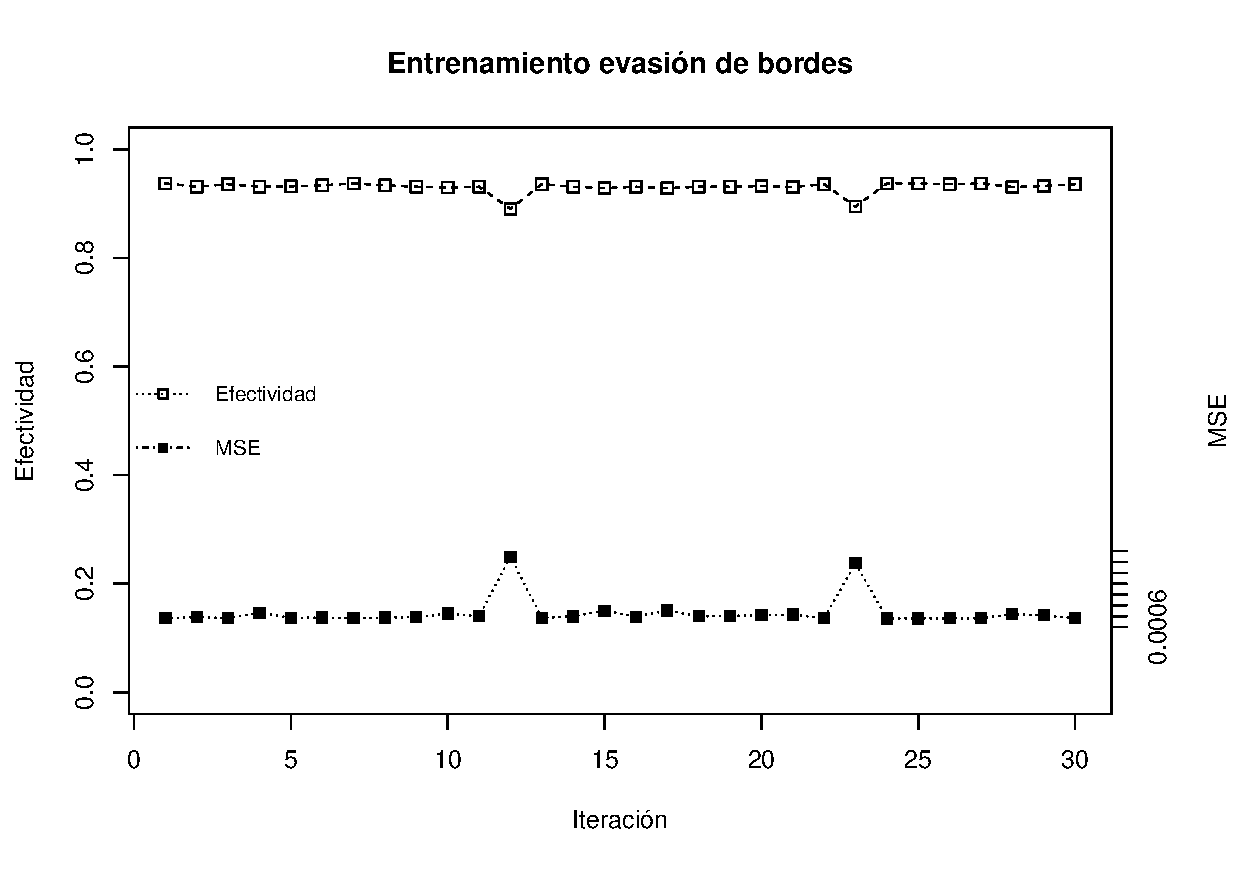
\includegraphics[width = 450pt]{images/plot_net_1_b.pdf}
  \caption[Entrenamiento primera etapa Red.1.B.]{Resultado del entrenamiento después de 30 iteraciones de Red.1.B.}
  \label{fig:net.1.b}
\end{figure}

Como se puede ver en las figuras no existe mucha diferencia en la efectividad de las dos redes, las dos tiene una efectividad máxima de 0.9370164, en la figura \ref{fig:net.1.a vs net.1.b} se muestra la comparación entre las dos redes. A través de las 30 iteraciones la desviación estándar de la efectividad de Red.1.A es de 0.01846731 y de Red.1.B es 0.01068135.\\

Dado que las dos redes tiene un número distinto de neuronas se diferencia en el tiempo que se tarda en computar el entrenamiento, Red.1.A toma 2.7691 minutos en completar las 30 iteraciones y Red.1.B 8.4236 minutos.\\

El MSE de las redes es bastante bajo, en comparación con un resultado aleatorio que presenta un valor de 0.25, a lo largo del entrenamiento el MSE máximo y mínimo de Red.1.A es de 0.00069 y 0.001812, el de Red.1.B de 0.00067 y 0.00124.\\


\begin{figure}[H]
  \centering
  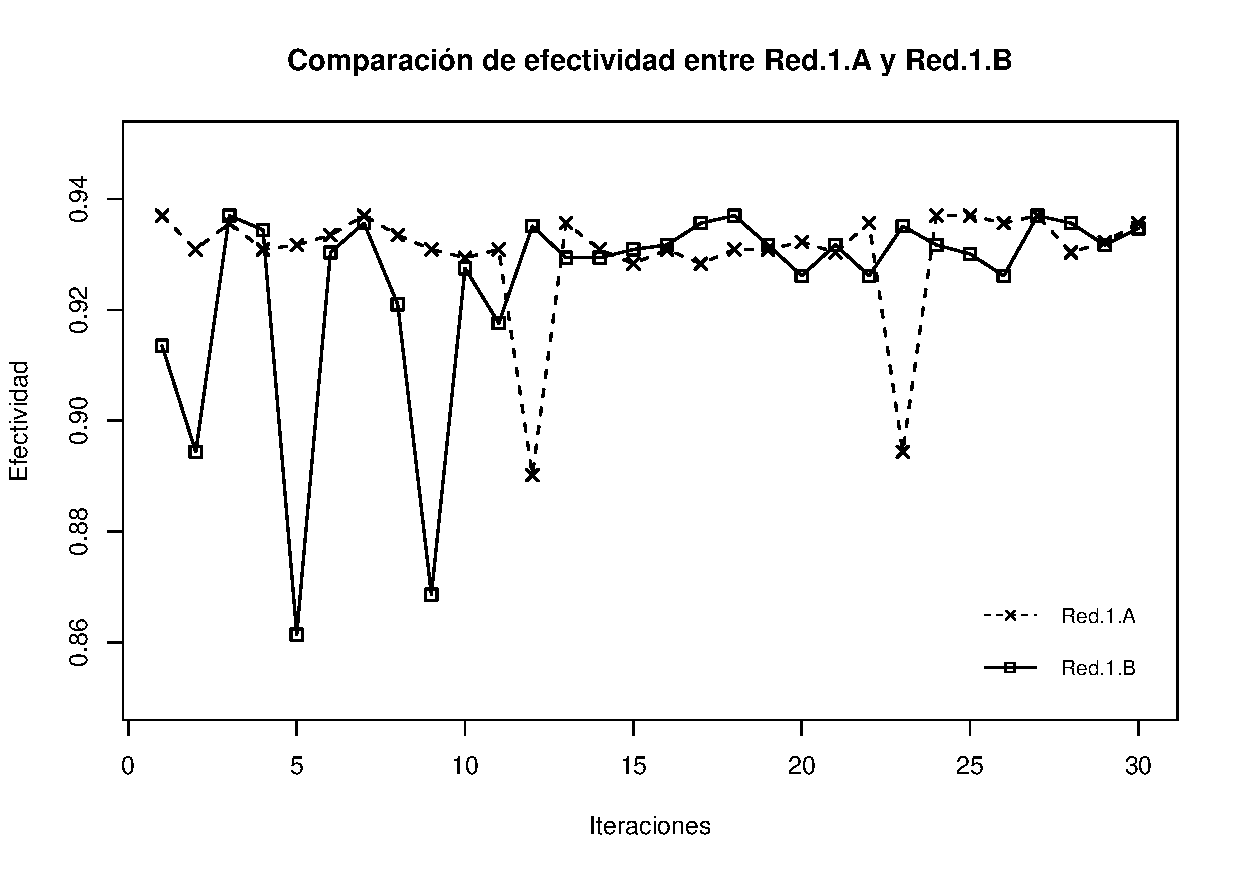
\includegraphics[width = 450pt]{images/net_1_a_vs_net_1_b.pdf}
  \caption[Efectividad de Red.1.A vs Red.1.B.]{Comparación de efectividad entre Red.1.A y Red.1.B.}
  \label{fig:net.1.a vs net.1.b}
\end{figure}

En la tabla \ref{tab:Red.1.A vs Red.1.B} muestra una comparativa entre el entrenamiento de las redes neuronales Red.1.A y Red.1.B.\\

\begin{table}[H]
\caption{Datos comparativos del entrenamiento en Red.1.A  y Red.1.B}
\makebox[\textwidth][c]{	
	\fontfamily{cmss}\selectfont{
	\begin{tabular}{c|ccccc}
	\addlinespace
	\toprule
	{\bf } & \multicolumn{ 5}{|c}{{\bf Entrenamiento Red.1.A y Red.1.B}} \\
	\midrule
	{\bf Red} & {\bf Efectividad} & {\bf Desviación} & {\bf MSE minimo} & {\bf MSE maximo} & {\bf Tiempo de} \\
	& {\bf maxima} & {\bf estándar} & & & {\bf entrenamiento}\\
	Red.1.A & 0.9370164 & 0.01846731 & 0.0006908158 & 0.0018120270 & 2.76913118362\\
	Red.1.B & 0.9370164 & 0.01068135 & 0.0006799585 & 0.0012468020 & 8.42360328436\\
	\bottomrule
	\end{tabular}
	}
}
\label{tab:Red.1.A vs Red.1.B}
\end{table}

\subsection{Evasión de obstaculos}

En esta etapa se utilizan los mismos datos que en la evasión de bordes, pero a estos se le suman 31542 elementos al set de entrenamiento y 13268 al de validación, obtenidos de los recorridos realizados por la conducción del robot evadiendo obstáculos. Con estos nuevos conjuntos de datos que tienen un total de 66297 elementos para el entrenamiento y 20635 para la validación, se vuelve a hacer el proceso de entrenamiento, iterar 30 veces para ambas redes neuronales (denotadas como Red.2.A y Red.2.B) y al término de cada entrenamiento hacer la comprobación con los datos de validación. La figura \ref{fig:net.2.a} y \ref{fig:net.2.b} muestra los resultados del proceso.\\

Al igual que en la primera etapa no se muestra mucha diferencia entre la efectividad de las redes neuronales Red.2.A y Red.2.B, pero esta vez las red que cuenta con más neuronas, Red.2.B, logró una efectividad de 0.932348 mientras que Red.2.A 0.9311849, la figura \ref{fig:net.2.a vs net.2.b} muestra una comparativa entre las dos. La desviación estándar a lo largo del entrenamiento fue de 0.01630602 y 0.001632309, para la Red.2.A y Red.2.B respectivamente. Además ambas redes disminuyeron su resultados en comparación con el primera etapa, pero destaca la Red.2.B por tener una disminución notoria frente a las demás redes.\\

Debido al aumento tanto del set de datos de entrenamiento como el de validación los tiempos para completar el entrenamiento también aumentaron siendo de 5.5678 minutos para Red.2.A y 17.6041 para Red.2.B. Nuevamente debido al número de neuronas el tiempo de entrenamiento es mayor para la segunda red.\\

\begin{figure}
  \centering
  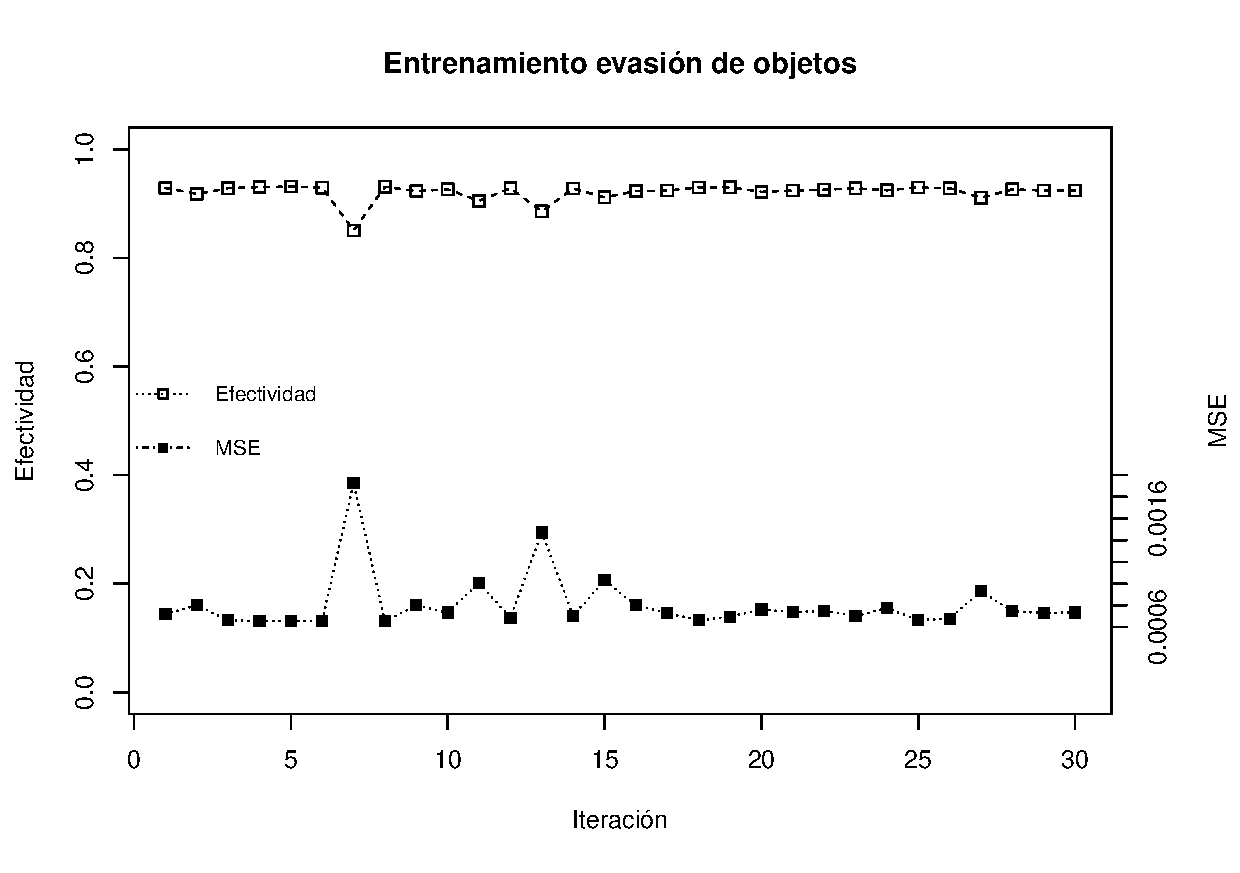
\includegraphics[width = 450pt]{images/plot_net_2_a.pdf}
  \caption[Entrenamiento segunda etapa Red.2.A.]{Resultado del entrenamiento después de 30 iteraciones de Red.2.A.}
  \label{fig:net.2.a}
\end{figure}

\begin{figure}
  \centering
  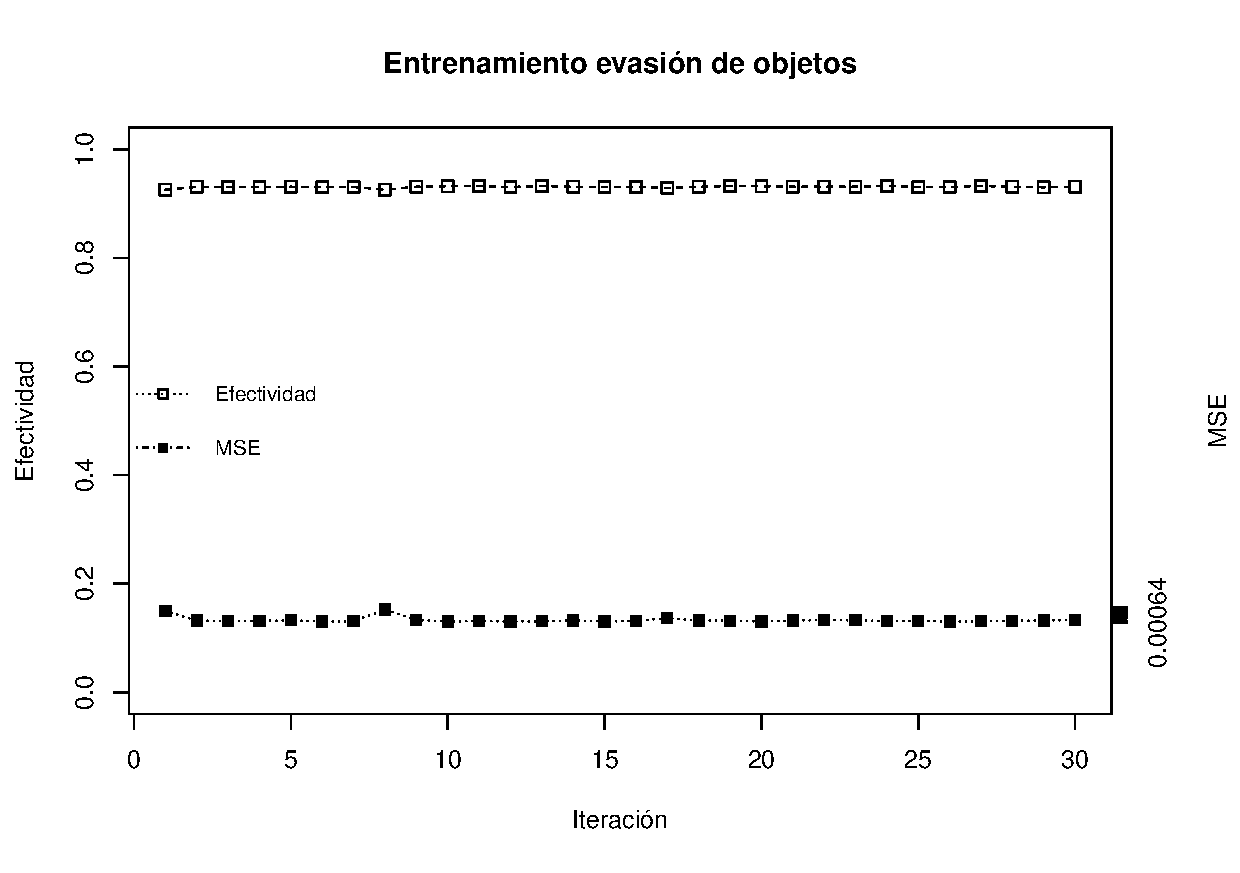
\includegraphics[width = 450pt]{images/plot_net_2_b.pdf}
  \caption[Entrenamiento segunda etapa Red.2.A.]{Resultado del entrenamiento después de 30 iteraciones de Red.2.b.}
  \label{fig:net.2.b}
\end{figure}

El MSE en esta etapa también se mantuvo con valores bajos, pero al igual que la desviación estándar de la Red.2.B el rango sufrió una reducción notoria, siendo de 0.0006519474 y 0.0007619559 mientras que para la Red.2.A el mínimo y máximo fue de 0.000653724 y 0.001927609 respectivamente.\\

\begin{figure}[H]
  \centering
  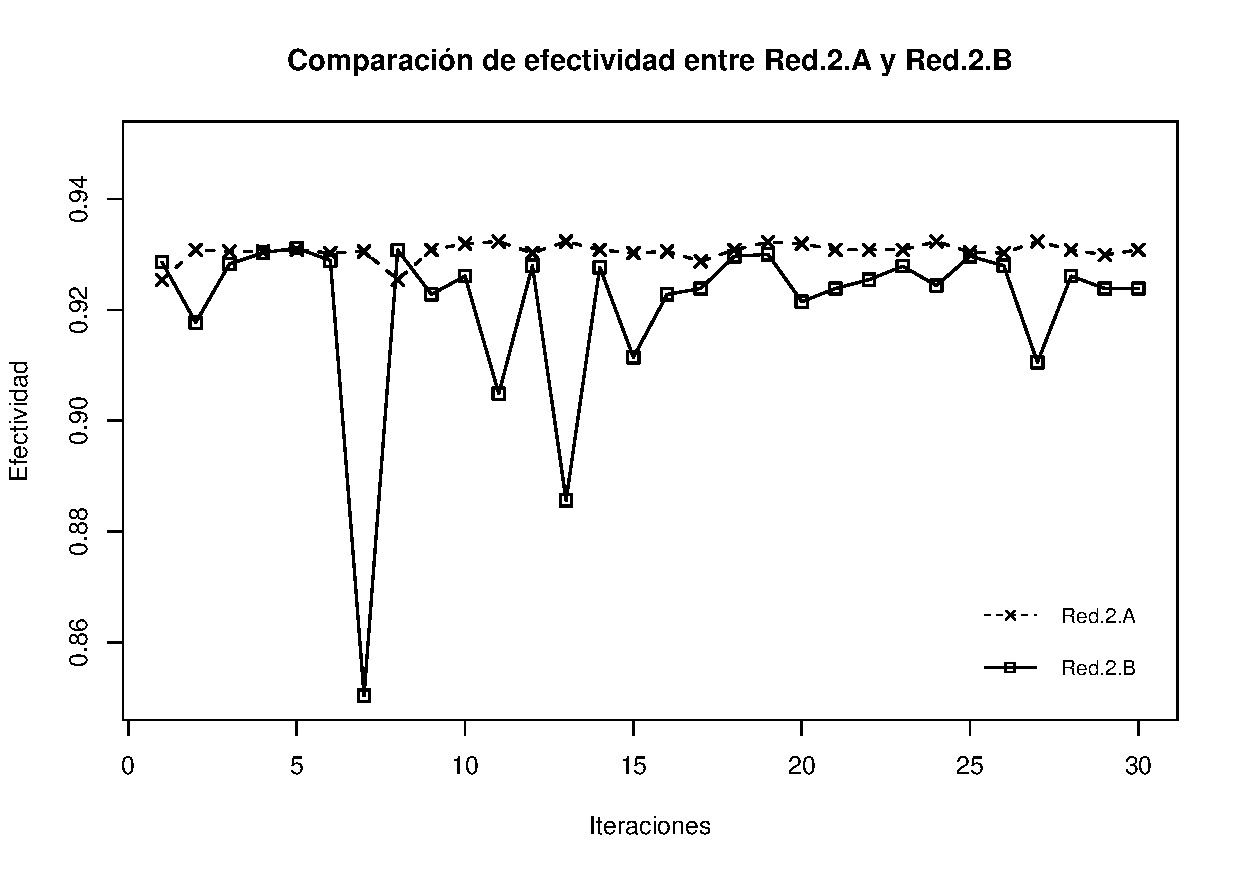
\includegraphics[width = 450pt]{images/net_2_a_vs_net_2_b.pdf}
  \caption[Efectividad de Red.2.A vs Red.2.B.]{Comparación de efectividad entre Red.2.A y Red.2.B.}
  \label{fig:net.2.a vs net.2.b}
\end{figure}

La tabla \ref{tab:Red.2.A vs Red.2.B} muestra la comparativa entre la Red.2.A y Red.2.B de los resultados obtenidos en la segunda etapa de entrenamiento.\\

\begin{table}[H]
\caption{Datos comparativos del entrenamiento en Red.2.A  y Red.2.B}
\makebox[\textwidth][c]{	
	\fontfamily{cmss}\selectfont{
	\begin{tabular}{c|ccccc}
	\addlinespace
	\toprule
	{\bf } & \multicolumn{ 5}{|c}{{\bf Entrenamiento Red.2.A y Red.2.B}} \\
	\midrule
	{\bf Red} & {\bf Efectividad} & {\bf Desviación} & {\bf MSE minimo} & {\bf MSE maximo} & {\bf Tiempo de} \\
	& {\bf maxima} & {\bf estándar} & & & {\bf entrenamiento}\\
	Red.2.A & 0.9311849 & 0.01630602 & 0.000653724 & 0.001927609 & 5.56788144906\\
	Red.2.B & 0.932348 & 0.001632309 & 0.0006519474 & 0.0007619559 & 17.604199481\\
	\bottomrule
	\end{tabular}
	}
}
\label{tab:Red.2.A vs Red.2.B}
\end{table}

En el anexo \ref{appendix:entrenamiento red} se muestran los resultados completos del entrenamiento realizado a las distintas redes neuronales, se listan las iteraciones y en cada una la efectividad y MSE conseguidos.\\

\section{Conducción autonoma}

Una vez que se terminó de entrenar las redes neuronales se probó la capacidad que estas tenían de conducir el robot por la pista de pruebas. Primero se prueba sin ningún objeto que evadir, el robot sólo tiene que dirigirse por el centro de la pista, con el objetivo de replicar el comportamiento de la conducción manual.\\

Al momento de realizar la primera prueba se registra que el robot no reacciona frente al flujo óptico, sin importar la información que recibe el comportamiento de este es el mismo, no cambia la dirección de la trayectoria. La respuesta que entrega la red debería modificar el recorrido en el eje $X$ de la pista, pero en la prueba la información que se le entrega al robot indica que este no debe realizar ningún movimiento. Esto se traduce en que el movimiento siempre es en línea recta.\\

El resultado obtenido se repitió con las dos redes entrenadas, tanto con Red.1.A como Red.1.B, la salida de la red está normalizada entre 0 y 1, cuando toma el valor mayor a 0.5 el robot debe moverse a la derecha, si el valor es menor a la izquierda y si permanece en 0.5 la dirección no debe cambiar. La salida analizada siempre se mantenía en 0.5 o muy cercana a este valor, sin importar el flujo óptico que se utilizaba como entrada para la red.\\

Dado el comportamiento obtenido con la utilización de la red neuronal para la conducción autónoma se puede considerar que la prueba fue fallida, aunque los resultados de la validación de entrenamientos haya sido exitosos.\\

\section{Análisis}

Como se deja ver en los resultados obtenidos existe una contradicción entre la validación del entrenamiento de la red y la conducción autónoma, por esta razón se revisa la forma en que se realiza el entrenamiento. Este tiene una estrecha relación con los datos capturados, los que son el flujo óptico y los movimientos del robot, ambos capturados de los recorridos hechos en la pista de prueba.\\

Los movimientos del robot que son capturados por el sensor de movimientos tiene un valor mínimo de -255 y máximo de 255, los que son normalizados entre 0 y 1. Estos registran el desplazamiento del robot sobre el eje $X$. Se analiza la distribución que tienen estos en los datos de entrenamiento.\\

\begin{figure}[H]
  \centering
  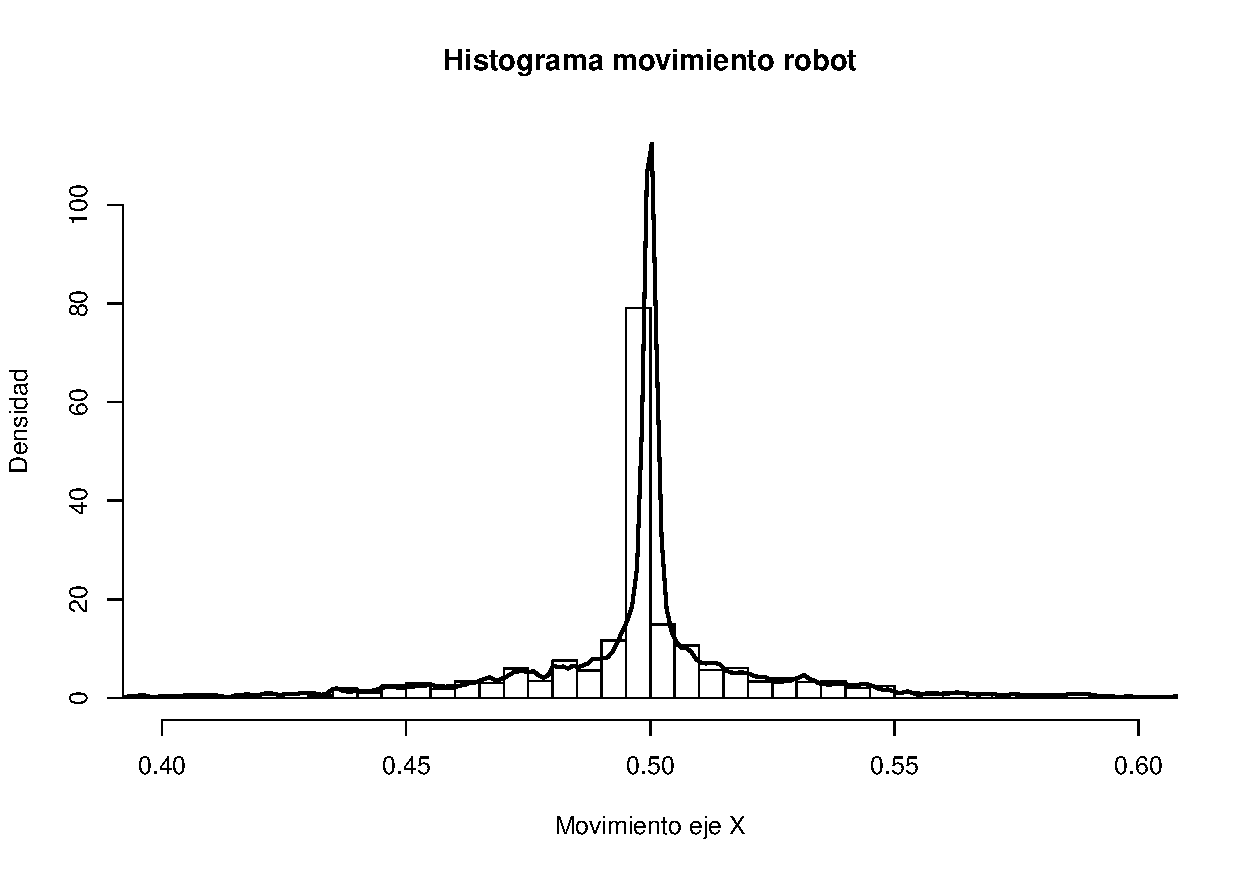
\includegraphics[width = 450pt]{images/hist_motion_robot.pdf}
  \caption[Histograma movimiento robot en el eje $X$]{Histogram del movimiento registrado en el desplazamiento del robot por el eje $X$ de la pista.}
  \label{fig:hist motion robot}
\end{figure}

En la figura \ref{fig:hist motion robot} se puede ver que la concentración de los datos se encuentra alrededor del valor 0.5, lo que significa que a lo largo de la captura de datos de entrenamiento no se registró el desplazamiento que hacía lateralmente el robot. Esto trae como consecuencia que al momento de hacer el entrenamiento la red aprende que indistintamente del flujo óptico que recibe como entrada la salida que debe entregar es 0.5.\\

\begin{figure}[H]
  \centering
  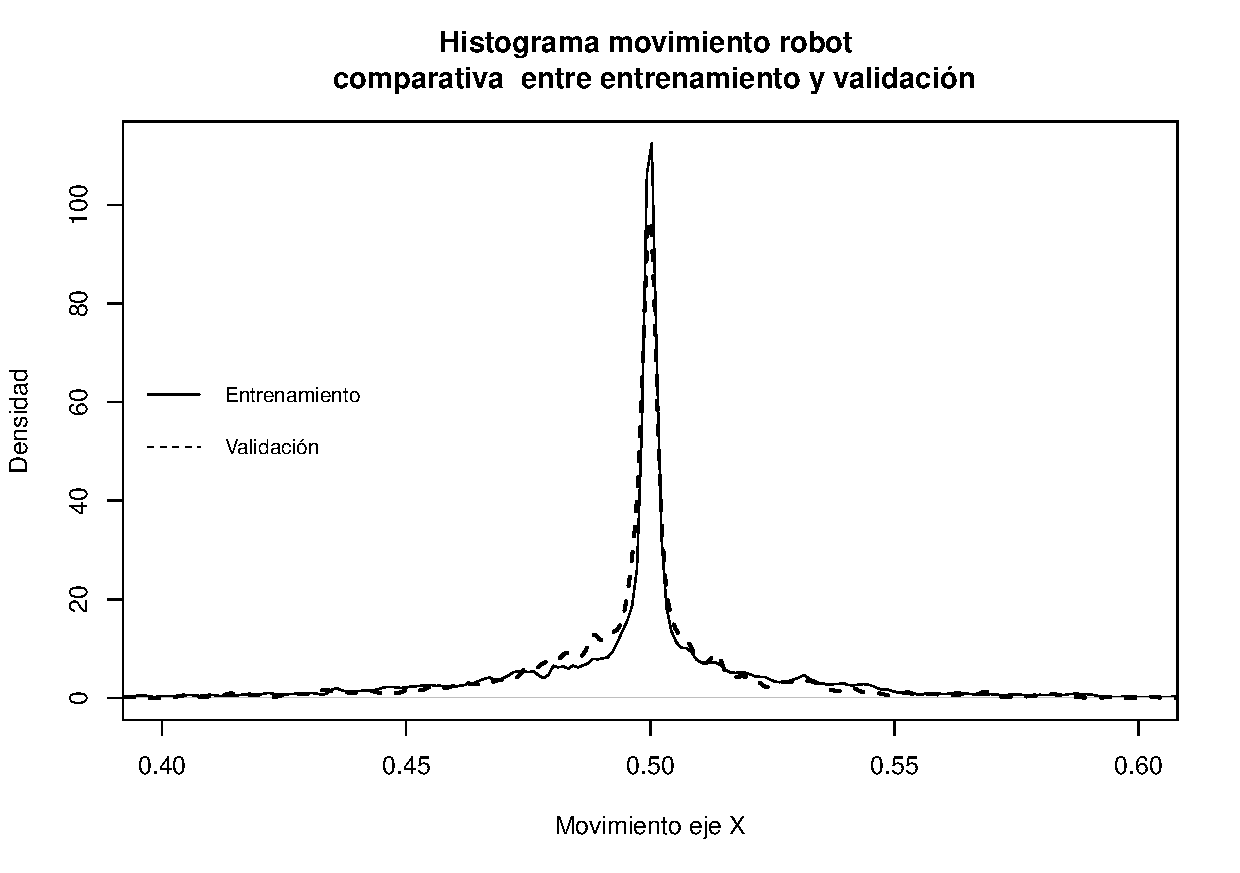
\includegraphics[width = 450pt]{images/hist_motion_robot_training_vs_test.pdf}
  \caption[Histograma movimiento robot entrenamiento v/s validación]{Comparativa de histogramas entre datos de entrenamiento y validación del movimiento registrado en el desplazamiento del robot por el eje X de la pista.}
  \label{fig:hist motion robot training test}
\end{figure}

Ahora si se analiza los datos para la validación del entrenamiento, se ve que estos tiene una distribución que concuerda con los datos con que se realizó el entrenamiento, figura \ref{fig:hist motion robot training test} muestra la comparativa entre los datos de entrenamiento y validación. Es por esta razón que cuando se valida el entrenamiento el resultado obtenido es una alta efectividad, a pesar de que el entrenamiento no cumple con el objetivo que se busca.\\

Las razones por la que se obtuvieron estos datos están estrechamente relacionados con el sensor óptico de movimiento, el desplazamiento hecho por el robot en el intervalo de dos \emph{frames} consecutivos pudo ser captado como un movimiento muy pequeño o nulo por el sensor. Otro motivo por el cual no se registraron los datos esperados es que el sensor no puedo captar el movimiento por no estar funcionando bajo las especificaciones para las que fue diseñado, como el no estar en un tipo de superficie compatible o estar fuera del rango de distancia que se necesita para captar el movimiento relativo a la superficie donde se desplaza.\\

\begin{figure}[H]
  \centering
  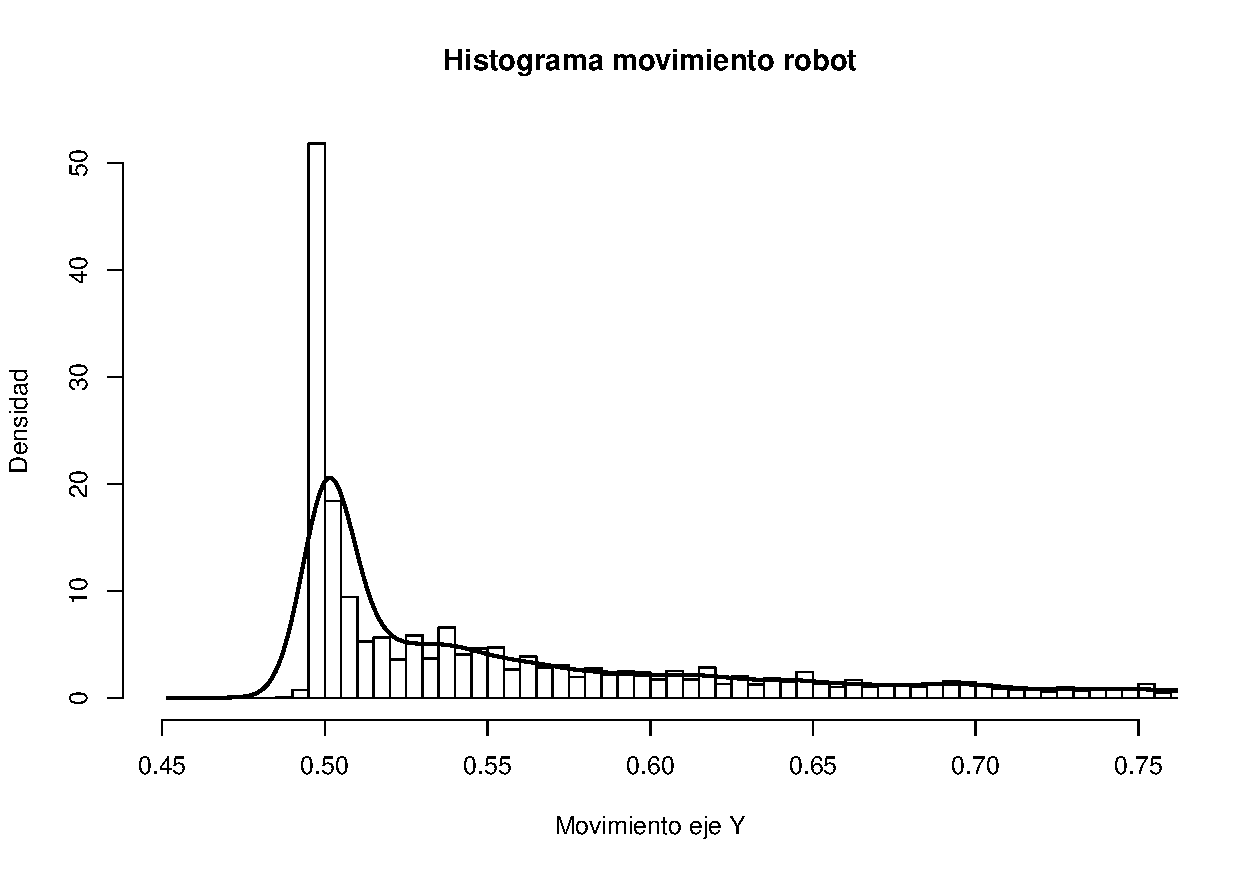
\includegraphics[width = 450pt]{images/hist_motion_robot_y.pdf}
  \caption[Histograma movimiento robot en eje $Y$]{Histogram del movimiento registrado en el desplazamiento del robot por el eje $Y$ de la pista.}
  \label{fig:hist motion robot y}
\end{figure}

Al analizar el movimiento del robot en el eje $Y$ gana más sustento el segundo motivo descrito anteriormente, al momento de capturar los datos el el robot siempre estuvo en movimiento sobre este eje, por lo que el sensor nunca debió entregar un valor de 0.5 ya que esto significa que robot no se está desplazando. Al ver los datos del sensor se puede apreciar que al igual en el eje $X$ la mayor concentración está alrededor del valor 0.5, la figura \ref{fig:hist motion robot y} muestra la distribución que estos tuvieron.\\

Teniendo estos antecedentes en cuenta se puede concluir que efectivamente al momento de capturar los datos, tanto de entrenamiento como de validación, no se capturó adecuadamente el movimiento del robot. El sensor de movimiento en la mayoría de los casos no alertó desplazamiento alguno cuando en la realidad el robot estuvo en constante movimiento mientras se obtenían los datos.\\

Este fallo en la percepción de movimiento del robot no fue alertado con anterioridad por tener en pruebas preliminares buenos resultados en la validación del entrenamiento. Esos resultados no sugieren tener una falencia en los datos utilizados para entrenar red neuronal. Tampoco se contaba con una retroalimentación visual de la cuantificación del desplazamiento como si se tenía de la captura de flujo óptico.\\

Para corregir esta falencia es necesario hacer un rediseño en el robot omnidireccional que permita un buen funcionamiento del sensor de movimiento, garantizando que cualquier movimiento hecho por este pueda ser percibido por el sensor. Otra opción es utilizar un tipo diferente de sensor que se adapte mejor a los requerimientos específicos de cuantificar el desplazamiento hecho por el robot.\\

En este capítulo se expusieron los resultados obtenidos de las distintas pruebas realizadas, las que consistieron en evaluar el entrenamiento de la red neuronal y cómo se comportaba el robot en la conducción autónoma, además de analizar el porqué de los resultados.\\

\chapter{Conclusión}

En este capitulo se revisa el trabajo realizado desde el punto de vista de los planteamientos hechos en un comienzo y si fue posible cumplir con estos. Se revisan los objetivos planteados, como fueron abordados y si pudieron ser completados.\\

Además de exponer las experiencias que se tuvieron a lo largo de la implementacion de la solución y el porqué se abordo la problematica de esta forma.\\

Para finalmente ver cual es el trabajo que queda pendiente y que cosas se podrian hacer en el futuro para ampliar el ambito de la solución.\\

\section{Objetivos}

Con todos los antecedentes recopilados y redactados en este documento no es posible decir que se logró cumplir con el objetivo principal que se planteó, debido a las razones argumentadas anteriormente. Por otro lado no se descarta que la solución planteada pueda llevarse a cabo si se redefinen ciertos puntos de la implementación, que son necesarios para resolver la problemática, haciendo referencia a falencia de la captura de movimiento del robot.\\

Ahora si se revisan los objetivos específicos, que desglosan el trabajo realizado durante la construcción de la solución a la problema planteada se puede decir lo siguiente:


\begin{itemize}
	\item {\bf Definir herramientas que permitan la obtención del flujo óptico desde la captura de video}: Este era un de los objetivos principales de solución, marca el punto de partida para el resto de la implementación que se trabajó posteriormente. Se logró desarrollar el \emph{software} necesario para calcular el flujo óptico, teniendo que indagar y comprender el funcionamiento de algoritmos de procesamiento de imágenes, como lo es el método \emph{Lucas-Kanade}. Con esto se logró diseñar una solución, con la que podemos decir que este objetivo fue cumplido.\\
	
	\item {\bf Implementación de una red neuronal que permita el procesamiento del flujo óptico:} Las investigaciones que se realizaron permitieron encontrar una implementación de una red neuronal que pudo ser adaptada a las necesidades específicas de este trabajo. Apesar de que era un trabajo ya desarrollado de todos modos fue necesario hacer un estudio detallado de cómo fue realizada esta implementación y analizar su funcionamiento. El cumplimiento de este objetivo implica a su vez manipular la información obtenida del flujo óptico, ya que no basta  solo con la obtención de datos, sino que es necesaria la adaptación de estos para lograr el trabajo en conjunto con la red neuronal. Permitiendo poder procesar el flujo óptico por medio de una red neuronal.\\
	
	\item {\bf Entrenamiento de una red neuronal para que sea capaz de aprender cómo evadir obstáculos:} Si bien se logró llevar a cabo el entrenamiento de una red neuronal mediante datos obtenidos del cálculo de flujo óptico, este entrenamiento no dio los resultados esperados, a pesar de que la cuantificación obtenida cumplia con las metricas definidas para dar este como exitoso. Esto muestra que a pesar de tener buenos resultados estos no siempre son los que se necesitan o son los que permitirán cumplir con los objetivos planteados. Por las pruebas hechas posteriormente se pudo determinar que este objetivo no pudo ser cumplido.\\
	
	\item {\bf Implementación de un robot omnidireccional que permite la obtención de datos para entrenar la red neuronal:} Este objetivo es el que necesito mayor trabajo para ser completado. Abarca distintas áreas interdisciplinarias ya que el diseño tomó solo algunas referencias a elementos ya construidos y desde estas se realizó el diseño y construcción completa del robot. Fue necesaria la aplicación de diversos conocimientos como: modelado 3D, fabricación de piezas por impresión 3D, electrónica de microcontroladores y desarrollo de software, entre otros. Logrando así la construcción de una herramienta que además puede ser utilizada en el desarrollo de futuras investigaciones en este u otros ámbitos.\\
	
	\item {\bf Realizar pruebas con el robot para evaluar el comportamiento de la red neuronal ante obstáculos:} Este objetivo es el que permite determinar si fue o no posible dar como exitoso el objetivo principal. Además de aglomerar todo el trabajo realizado. Una vez construido el robot y hecho el entrenamiento pertinente a la red neuronal se necesita saber si en conjunto pueden servir de solución al problema planteado, lo que se logra por medio del desarrollo de pruebas y posterior análisis de resultados. Estos dejaron en evidencia una falencia que compromete el cumplimiento del objetivo principal, pero a su vez permitieron dar con un diagnóstico y posibles soluciones para poder llegar a cumplir el objetivo. Si bien el robot cumple con su función de realizar las pruebas necesarias los resultados obtenidos no fueron los esperados. Estos dan a conocer que el entrenamiento realizado no permite la evasión de obstáculos por medio de la conducción autónoma del robot.\\
\end{itemize}

\section{Trabajo realizado}

Un punto importante fue la motivación que llevó el desarrollo de la solución planteada, la cual fue tomar como referencia elementos que existen en la naturaleza. Partir de esos referentes y usarlos como ejemplo para traspasar esos conceptos por medio de la construcción de un sistema que imite el desempeño de algunas entidades biológicas. El punto central indaga en el funcionamiento de las conexiones que hacen las neuronas para poder procesar informacion, de esto se basa la utilización de redes neuronales para analizar otro elemento que proviene de la naturaleza que es el flujo óptico. Todo esto culmina con la construcción de un robot que no solo pretende tener conducción autónoma, sino que busca ser un reflejo de lo el mundo natural puede hacer.\\

Sin dudas esto lleva a un objetivo ambicioso pero que buscaba abarcar otras áreas que no son cubiertas o por lo menos no en profundidad en la formación profesional. Si bien el desempeño como ingeniero civil en computación cumple un rol fundamental de forma transversal en toda la implementación de este proyecto, también quise añadir otras áreas que estuvieran fuera del ámbito central que se estudia a lo largo de carrera y que son se mi interés, como lo es la computación física. Para mi es muy llamativo el diseño de elementos que puedan interactuar de forma más tangible en nuestro entorno, como lo es la construcción de robots, estos permiten la unión del conocimiento adquiridos de los estudios como los aprendidos de forma autónoma por simple motivación.\\

A medida que se iba avanzando en el cumplimientos de los objetivos, fue posible darse cuenta de las diferencias que existen en la construcción de elementos que son abstractos en comparación con la implementaciones de objetos que tiene que lidiar con el mundo físico. La forma acostumbrada trabajar es tomar un idea, modelarla y plasmarla como una pieza de software, sin embargo cuando se parte de la misma base pero esta tiene que ser implementada y construida físicamente, esta no se comporta como uno espera o no puede prever los inconvenientes que pueden surgir. En contraste con el desarrollo de \emph{software} donde se trabaja en un ambiente que es controlado y se conocen todas la variables que influyen en su comportamiento. Esto llevó a distintos eventos no anticipados en los que se debió buscar soluciones para poder seguir adelante con el desarrollo, sin embargo situaciones como esas comprometieron el cumplimiento de objetivos planteados.\\

Por último, si bien no se obtuvieron los resultados esperados, de todos modos fue satisfactorio el trabajo realizado, ya que durante este fue necesario conocer sobre nuevas áreas, como por ejemplo los cuadricópteros, además de concluir la construcción del robot omnidireccional, el que no solo forma parte de este ámbito en particular, sino que puede ser utilizado como una herramienta para trabajar en proyectos futuros.\\

\section{Trabajo futuro}

Debido a que quedaron elementos pendientes en los objetivos planteados, en primer lugar se deben solucionar los problemas encontrados, para que de esta forma se puedan volver a efectuar las pruebas planteadas y obtener los resultados esperados. Por otro lado debido a los ámbitos especificados falta la construcción de nuevos elementos que permitan en un futuro poder implementar este sistema en vehículos aéreos no tripulados y de esta forma poder dar un solución al problema planteado.\\

Dentro de estos elementos está por ejemplo ampliar las pruebas a condiciones más complejas, como evadir múltiples objetos en más de una dirección y que puedan estar en movimiento, también poder portar el sistema al \emph{hardware} adecuado para que este, por ejemplo, pueda funcionar a bordo de un cuadricóptero y ver cómo se comporta el sistema en una situación real.\\

También sería de interés poder ampliar el sistema para que pueda trabajar no solo con la información proveniente del flujo óptico, si no que poder contar una red neuronal que sea capaz de procesar distintos tipos de información a la vez y de estar forma poder agregar mayor capacidad al sistema planteado.\\

Otra alternativa es expandir el ámbito en el cual se planteó el problema y no solo usar el sistema para mejorar la autonomía de los vehículos aéreos no tripulados, si no que analizar en qué otra áreas podría ser de utilidad, por ejemplo, como asistencia a personas con visión reducida para puedan desplazarse con mayor facilidad.\\

%% ambiente glosario
\begin{glosario}
	\item[Ángulo de ataque:] Se denomina ángulo de ataque al ángulo que forman la cuerda geométrica de un perfil alar con la dirección del aire incidente.
	\item[Caja reductora:]  Mecanismo que consiste en un grupo de engranajes con el que se consigue reducir el número de revoluciones.
	\item[Circuito en serie:] Un circuito en serie es una configuración de conexión en la que los bornes o terminales de los dispositivos se conectan secuencialmente. La terminal de salida de un dispositivo se conecta a la terminal de entrada del dispositivo siguiente.
	\item[Filtro gaussiano:] Un filtro gaussiano es un filtro cuyo impulso es una función gaussiana
	\item[Grado de libertad:] Grados de libertad se refiere al número mínimo de parámetros que necesitamos especificar para determinar completamente la velocidad de un mecanismo o el número de reacciones de una estructura.
	\item[Holonómico:] Sistemas holonómicos son aquellos capaces de modificar su dirección instantáneamente y sin necesidad de rotar previamente.
	\item[Impresión 3D:] La impresión 3D es un grupo de tecnologías de fabricación por adición donde un objeto tridimensional es creado mediante la superposición de capas sucesivas de material
	\item[LED:] LED del inglés: \emph{light-emitting diode} (diodo emisor de luz) es un componente optoelectrónico activo y, más concretamente, un diodo que emite luz.
	\item[Modelado Paramétrico:] Se denomina diseño paramétrico a un proceso de diseño basado en un esquema algorítmico que permite expresar parámetros y reglas que definen, codifican y aclaran la relación entre los requerimientos del diseño y el diseño resultante.
	\item[Motor DC:] El motor de corriente continua es una máquina que convierte energía eléctrica en mecánica, provocando un movimiento rotatorio, gracias a la acción de un campo magnético.
	\item[Open source:] El software de código abierto (en inglés open source) es el software cuyo código fuente y otros derechos que normalmente son exclusivos para quienes poseen los derechos de autor, son publicados bajo una licencia de código abierto o forman parte del dominio público.
	\item[Overflow:] Ocurre cuando una operación aritmética intenta crear un valor numérico que está fuera del rango que se puede representar con un número dado de bits
	\item[Paso de hélice:] Es el angulo de ataque que forma la helice con respecto a vector de movimiento del aire.
\end{glosario}


%% genera las referencias
\bibliography{refs}


%% comienzo de la parte de anexos
\appendixpart

%% contenido del primer anexo
\appendix{Resultados entrenamiento de redes neuronales}
\label{appendix:entrenamiento red}

\section{Red.1.A}

\begin{longtable}{ccc} 
\caption{Datos del entrenamiento realizado a la Red.1.A.}\label{tab:training Red.1.A}\\

	\addlinespace
	\toprule
	\multicolumn{3}{c}{{\bf Entrenamiento Red.1.A}} \\
	\midrule
	{\bf Iteración} & {\bf Efectividad} & {\bf MSE} \\
	1 & 0.913533324284 & 0.000945908778483 \\
	2 & 0.894393918827 & 0.00119303279299 \\
	3 & 0.937016424596 & 0.00069081575127 \\
	4 & 0.934437355776 & 0.00070042173591 \\
	5 & 0.861408986019 & 0.00181202704469 \\
	6 & 0.930365141849 & 0.000741045642054 \\
	7 & 0.935659019954 & 0.000691926551444 \\
	8 & 0.920999049817 & 0.000876352966901 \\
	9 & 0.868603230623 & 0.00167283443075 \\
	10 & 0.9275145921 & 0.000767064584306 \\
	11 & 0.917605538211 & 0.000846716155162 \\
	12 & 0.935116058097 & 0.000700496521621 \\
	13 & 0.929414958599 & 0.000734796869545 \\
	14 & 0.929414958599 & 0.000724355116221 \\
	15 & 0.930908103706 & 0.000707206147845 \\
	16 & 0.931722546491 & 0.000693620418216 \\
	17 & 0.935659019954 & 0.000694472906729 \\
	18 & 0.937016424596 & 0.000690996410918 \\
	19 & 0.931722546491 & 0.000695499916258 \\
	20 & 0.926157187458 & 0.000797349211209 \\
	21 & 0.931722546491 & 0.000691992846241 \\
	22 & 0.926157187458 & 0.000804536187667 \\
	23 & 0.935116058097 & 0.000704533339926 \\
	24 & 0.931722546491 & 0.000696808227387 \\
	25 & 0.93009366092 & 0.000745401931822 \\
	26 & 0.926157187458 & 0.000811712662915 \\
	27 & 0.937016424596 & 0.000691168580695 \\
	28 & 0.935659019954 & 0.000692704302926 \\
	29 & 0.931722546491 & 0.000697733637806 \\
	30 & 0.934708836704 & 0.000691069343532 \\
	\bottomrule

\end{longtable}

\section{Red.1.B}

\begin{longtable}{ccc} 
\caption{Datos del entrenamiento realizado a la Red.1.B.}\label{tab:training Red.1.B}\\

	\addlinespace
	\toprule
	\multicolumn{3}{c}{{\bf Entrenamiento Red.1.B}} \\
	\midrule
	{\bf Iteración} & {\bf Efectividad} & {\bf MSE} \\
	1 & 0.937016424596 & 0.000680479158646 \\
	2 & 0.930908103706 & 0.000693363879534 \\
	3 & 0.935659019954 & 0.000681495122213 \\
	4 & 0.930908103706 & 0.000732845982048 \\
	5 & 0.931722546491 & 0.000683404847922 \\
	6 & 0.933487172526 & 0.000688381137309 \\
	7 & 0.937016424596 & 0.000680450324945 \\
	8 & 0.933487172526 & 0.000687662533276 \\
	9 & 0.930908103706 & 0.000692330783035 \\
	10 & 0.929414958599 & 0.000724415835138 \\
	11 & 0.930908103706 & 0.000701182301275 \\
	12 & 0.890185964436 & 0.00124680202199 \\
	13 & 0.935659019954 & 0.000683446893253 \\
	14 & 0.930908103706 & 0.000698575037316 \\
	15 & 0.928329034885 & 0.000751828245677 \\
	16 & 0.930908103706 & 0.000696074099689 \\
	17 & 0.928329034885 & 0.000753517327056 \\
	18 & 0.930908103706 & 0.000698791474565 \\
	19 & 0.930908103706 & 0.000703277030309 \\
	20 & 0.932265508348 & 0.00070997250449 \\
	21 & 0.930365141849 & 0.000715367567923 \\
	22 & 0.935659019954 & 0.000681680637419 \\
	23 & 0.894393918827 & 0.00118822859392 \\
	24 & 0.937016424596 & 0.000679987713934 \\
	25 & 0.937016424596 & 0.000679958482945 \\
	26 & 0.935659019954 & 0.000681375297971 \\
	27 & 0.937016424596 & 0.000680985065225 \\
	28 & 0.930365141849 & 0.000717947488892 \\
	29 & 0.932265508348 & 0.000708196541166 \\
	30 & 0.935659019954 & 0.00068277419994 \\
	\bottomrule

\end{longtable}

\section{Red.2.A}

\begin{longtable}{ccc} 
\caption{Datos del entrenamiento realizado a la Red.2.A.}\label{tab:training Red.2.A}\\

	\addlinespace
	\toprule
	\multicolumn{3}{c}{{\bf Entrenamiento Red.2.A}} \\
	\midrule
	{\bf Iteración} & {\bf Efectividad} & {\bf MSE} \\
	1 & 0.928616428398 & 0.000719893721006 \\
	2 & 0.917712624182 & 0.000800126689279 \\
	3 & 0.928277198934 & 0.000664979822336 \\
	4 & 0.930312575721 & 0.000654552914366 \\
	5 & 0.931184880058 & 0.000654863604206 \\
	6 & 0.928907196511 & 0.000658793172797 \\
	7 & 0.850399806155 & 0.00192760902722 \\
	8 & 0.930797189242 & 0.000653724038728 \\
	9 & 0.92280106615 & 0.000800747839431 \\
	10 & 0.926096438091 & 0.000733538849396 \\
	11 & 0.904870365883 & 0.0010089428019 \\
	12 & 0.927986430821 & 0.000685578890759 \\
	13 & 0.885631209111 & 0.00147211690003 \\
	14 & 0.927695662709 & 0.000703759297938 \\
	15 & 0.911461109765 & 0.00103087829926 \\
	16 & 0.92280106615 & 0.000801065965672 \\
	17 & 0.923867215895 & 0.000730485527153 \\
	18 & 0.929682578144 & 0.000662293709483 \\
	19 & 0.930021807608 & 0.000696563117277 \\
	20 & 0.921492609644 & 0.000762692770483 \\
	21 & 0.923867215895 & 0.000737694338211 \\
	22 & 0.925466440514 & 0.000750068796091 \\
	23 & 0.927889508117 & 0.000701192146117 \\
	24 & 0.924400290768 & 0.000776208040826 \\
	25 & 0.929682578144 & 0.00066460162863 \\
	26 & 0.927986430821 & 0.000678062613667 \\
	27 & 0.910540344076 & 0.000930106000753 \\
	28 & 0.926096438091 & 0.000745957305927 \\
	29 & 0.923867215895 & 0.000730502893394 \\
	30 & 0.923867215895 & 0.000734406848618 \\
	\bottomrule

\end{longtable}

\section{Red.2.B}

\begin{longtable}{ccc} 
\caption{Datos del entrenamiento realizado a la Red.2.B.}\label{tab:training Red.2.B}\\

	\addlinespace
	\toprule
	\multicolumn{3}{c}{{\bf Entrenamiento Red.2.B}} \\
	\midrule
	{\bf Iteración} & {\bf Efectividad} & {\bf MSE} \\
	1 & 0.925417979162 & 0.000749432750139 \\
	2 & 0.930845650594 & 0.000660165282152 \\
	3 & 0.930554882481 & 0.000655959851093 \\
	4 & 0.930554882481 & 0.000656857864731 \\
	5 & 0.930845650594 & 0.000662295925217 \\
	6 & 0.930264114369 & 0.000652311348451 \\
	7 & 0.930554882481 & 0.000653654554964 \\
	8 & 0.925417979162 & 0.000761955863816 \\
	9 & 0.930845650594 & 0.000664555387331 \\
	10 & 0.931960261691 & 0.000652296703772 \\
	11 & 0.932347952508 & 0.000656277069034 \\
	12 & 0.930264114369 & 0.000652385361621 \\
	13 & 0.932347952508 & 0.000652944033472 \\
	14 & 0.930845650594 & 0.000661843223622 \\
	15 & 0.930264114369 & 0.000652187111804 \\
	16 & 0.930554882481 & 0.000656488882683 \\
	17 & 0.928761812455 & 0.000683020599665 \\
	18 & 0.930845650594 & 0.00066003563414 \\
	19 & 0.932251029804 & 0.00065971120924 \\
	20 & 0.931960261691 & 0.000651947403756 \\
	21 & 0.930845650594 & 0.000660280012452 \\
	22 & 0.930845650594 & 0.000665047738241 \\
	23 & 0.930845650594 & 0.000662555843386 \\
	24 & 0.932347952508 & 0.000654873962048 \\
	25 & 0.930409498425 & 0.00065689395976 \\
	26 & 0.930264114369 & 0.000652052591494 \\
	27 & 0.932347952508 & 0.0006534034983 \\
	28 & 0.930845650594 & 0.000657837034339 \\
	29 & 0.929924884904 & 0.000661217162169 \\
	30 & 0.930845650594 & 0.000664652371238 \\

	\bottomrule

\end{longtable}

\appendix{Arduino UNO rev 2}
\label{appendix:arduino uno}
Espesificaciones de la placa \emph{Arduino} UNO rev 2.

\begin{table}[H]
\caption[Especificaciones Arduino UNO.]{Especificaciones Arduino UNO.}
\centering
    \fontfamily{cmss}\selectfont{
    \begin{tabular}{|c|c|}

        \hline
            Microcontrolador & ATmega328P\\
        \hline
            Voltaje de operación & 5V\\
        \hline
            Voltaje de entrada (recomendado) & 7-12V\\
        \hline
            Voltaje de entrada (limite) & 6-20V\\
        \hline
            Pin digitales & 14 (6 proporcionan salida PWM)\\
        \hline
            Pin digitales PWM & 6\\
        \hline
            Pin de entrada analogica & 6\\
        \hline
            Corriente por pin & 20 mA\\
        \hline
            Corriente por pin 3.3V & 50 mA\\
        \hline
            Memoria Flash & 32 KBytes de los cuales 0.5 KBytes\\  & son usados por el bootloader\\
        \hline
            SRAM & 2 KBytes\\
        \hline
            EEPROM & 1 KBytes\\
        \hline
            Velocidad de reloj & 16 MHz\\
        \hline
            LED\_BUILTIN & 13\\
        \hline
            Largo & 68.6 mm\\
        \hline
            Ancho & 53.4 mm\\
        \hline
            Peso & 25 g\\
        \hline
    \end{tabular}
    }
\label{tab:arduino uno}
\end{table}


\appendix{Configuración impresora 3D}
\label{appendix:3D printer setting}
Configuración completa de la impresora 3D al momento de construir las piezas para el robot omnidireccional.

\begin{verbatim}

# generated by Slic3r 1.2.9 on Tue Jun 20 23:36:24 2017
avoid_crossing_perimeters = 0
bed_shape = 0x0,200x0,200x145,0x145
bed_temperature = 60
before_layer_gcode = 
bottom_solid_layers = 3
bridge_acceleration = 0
bridge_fan_speed = 100
bridge_flow_ratio = 1
bridge_speed = 30
brim_width = 0
complete_objects = 0
cooling = 1
default_acceleration = 0
disable_fan_first_layers = 3
dont_support_bridges = 1
duplicate_distance = 6
end_gcode = M104 S0 ; turn off temperature\nG28 X0  
; home X axis\nG0 Y149; \nM84     ; disable motors\n
external_fill_pattern = rectilinear
external_perimeter_extrusion_width = 0
external_perimeter_speed = 80%
external_perimeters_first = 0
extra_perimeters = 1
extruder_clearance_height = 20
extruder_clearance_radius = 20
extruder_offset = 0x0
extrusion_axis = E
extrusion_multiplier = 1
extrusion_width = 0
fan_always_on = 1
fan_below_layer_time = 0
filament_colour = #000000
filament_diameter = 1.75
fill_angle = 45
fill_density = 15%
fill_pattern = rectilinear
first_layer_acceleration = 0
first_layer_bed_temperature = 60
first_layer_extrusion_width = 250%
first_layer_height = 0.4
first_layer_speed = 50%
first_layer_temperature = 215
gap_fill_speed = 15
gcode_arcs = 0
gcode_comments = 0
gcode_flavor = reprap
infill_acceleration = 0
infill_every_layers = 1
infill_extruder = 1
infill_extrusion_width = 0
infill_first = 0
infill_only_where_needed = 0
infill_overlap = 15%
infill_speed = 40
interface_shells = 0
layer_gcode = 
layer_height = 0.2
max_fan_speed = 100
max_print_speed = 80
max_volumetric_speed = 0
min_fan_speed = 70
min_print_speed = 10
min_skirt_length = 0
notes = 
nozzle_diameter = 0.4
octoprint_apikey = 
octoprint_host = 
only_retract_when_crossing_perimeters = 1
ooze_prevention = 0
output_filename_format = [input_filename_base].gcode
overhangs = 1
perimeter_acceleration = 0
perimeter_extruder = 1
perimeter_extrusion_width = 0
perimeter_speed = 30
perimeters = 3
post_process = 
pressure_advance = 0
raft_layers = 0
resolution = 0
retract_before_travel = 2
retract_layer_change = 1
retract_length = 5
retract_length_toolchange = 10
retract_lift = 0
retract_restart_extra = 0
retract_restart_extra_toolchange = 0
retract_speed = 40
seam_position = aligned
skirt_distance = 6
skirt_height = 1
skirts = 2
slowdown_below_layer_time = 20
small_perimeter_speed = 15
solid_infill_below_area = 70
solid_infill_every_layers = 0
solid_infill_extruder = 1
solid_infill_extrusion_width = 0
solid_infill_speed = 80%
spiral_vase = 0
standby_temperature_delta = -5
start_gcode = G28 ; home all axes\n;G1 Z5 F5000 ; lift nozzle\n
support_material = 0
support_material_angle = 0
support_material_contact_distance = 0.2
support_material_enforce_layers = 0
support_material_extruder = 1
support_material_extrusion_width = 0
support_material_interface_extruder = 1
support_material_interface_layers = 3
support_material_interface_spacing = 0
support_material_interface_speed = 100%
support_material_pattern = pillars
support_material_spacing = 2.5
support_material_speed = 40
support_material_threshold = 0
temperature = 210
thin_walls = 1
threads = 2
toolchange_gcode = 
top_infill_extrusion_width = 0
top_solid_infill_speed = 50%
top_solid_layers = 3
travel_speed = 60
use_firmware_retraction = 0
use_relative_e_distances = 0
use_volumetric_e = 0
vibration_limit = 0
wipe = 0
xy_size_compensation = 0
z_offset = 0
\end{verbatim}

%% fin
\end{document}

   

